\chapter{Desarrollo del Proyecto}
En este capítulo se discute sobre el trabajo a realizado para la completitud del proyecto, así como la descripción y el post-mortem de las diferentes actividades realizadas durante su realización.

\section{Producto propuesto}
El producto desarrollado fue un videojuego multijugador. En este los alumnos pueden aprender conceptos básicos de los lenguajes de programación, viendo los conceptos de programación estructurada, mediante acertijos que les permitan de otra manera analizar su funcionamiento. En este juego se enfocó a la enseñanza de: variables, condicionales, ciclos y funciones, tratando temas de programación estructurada, basado en el material del curso de Fundamentos de la Programación y Programación I de la Universidad Autónoma de Ciudad Juárez, así como los libros Fundamentos de programación: Algoritmos, estructura de datos y objetos de Luis Joyanes Aguilar y Prelude to Programming: Concepts and design de Steward Venit y Elizabeth Drake. 
Las mecánicas del juego fueron inspiradas en el videojuego \textit{Among Us}. En este juego, un grupo de máximo 10 jugadores están juntos en una partida, hay una variedad de mapas y el punto es realizar todas las actividades que tienen asignadas para ganar. Pero del grupo de jugadores, unos cuantos son asignados como impostores y su trabajo es matar a los demás jugadores. Sin embargo, los jugadores pueden reportar muertes o sonar una alarma que les permite discutir y votar por quien es impostor, si sacan a todos los impostores, ganan los \textit{crewmates}, los jugadores no impostores.
El videojuego tendrá una duración aproximada de 20-30 minutos.

\section{Forma de validación}
Para la evaluación de la eficacia del producto creado se realizó en dos etapas.

\begin{itemize}
    \item Se pidió ayuda a un docente que en el semestre agosto-diciembre de 2021 impartiera clases de Fundamentos de Programación o de Programación 1. [TBD quien] Esto con el fin de validar el contenido por su valor didáctico, que cumpla las demandas del curso y enseñe el tema de manera correcta.
    \item Una vez evaluado el contenido, se probó con uno de los grupos que imparte este docente. Primero se hizo un pequeño examen/encuesta para evaluar su conocimiento, así como obtener su expectativa del juego antes que lo probaran. Después se puso en grupos de ocho jugadores a jugar. Y una vez terminada la partida, se puso a que contestaran una segunda encuesta, a fin de evaluar su conocimiento después del juego, así como obtener retroalimentación sobre problemas de usabilidad que encontraron y si el juego se les hizo divertido.
\end{itemize}

\section{Metodología}
\begin{longtable}[c]{|m{5cm}|c|c|c|}
\caption{Actividades del proyecto \label{table:fechas_actividades}}\\
\hline
Actividades                                         & Fecha de inicio & Fecha de termino   & Duración \\
\hline
Jugador puede agendar reuniones                    & 3-Feb-21  & 4-Feb-21  & 1      \\
\hline
Poder unirse a un lobby                            & 17-Dec-20 & 19-Dec-20 & 2      \\
\hline
Jugador puede moverse por el mapa                  & 2-Jan-21  & 2-Jan-21  & 0      \\
\hline
Jugador puede interactuar con objetos de la escena & 3-Jan-21  & 3-Jan-21  & 0      \\
\hline
Jugador puede votar por un jugador como culpable   & 24-Jan-21 & 2-Feb-21  & 9      \\
\hline
Moverse por las alcantarillas                      & 4-Feb-21  & 5-Feb-21  & 1      \\
\hline
Ocultar gente muerta                               & 5-Feb-21  & 5-Feb-21  & 0      \\
\hline
Votar por asesinos para expulsarlos                & 6-Feb-21  & 7-Feb-21  & 1      \\
\hline
Puzzle boilers -int                                & 8-Feb-21  & 8-Feb-21  & 0      \\
\hline
Puzzle de secuencia                                & 9-Feb-21  & 10-Feb-21 & 1      \\
\hline
Puzzle de variable-bool                            & 11-Feb-21 & 11-Feb-21 & 0      \\
\hline
Puzzle auto do-while                               & 12-Feb-21 & 12-Feb-21 & 0      \\
\hline
Puzzle variable-float                              & 12-Feb-21 & 13-Feb-21 &        \\
\hline
Puzzle cuarto de lavado -for                       & 14-Feb-21 & 14-Feb-21 & 0      \\
\hline
Puzzle zaguán- llenar cubeta -while                & 15-Feb-21 & 15-Feb-21 & 0      \\
\hline
Puzzle if                                          & 16-Feb-21 & 16-Feb-21 & 0      \\
\hline
Puzzle string-substring                            & 17-Feb-21 & 17-Feb-21 & 0      \\
\hline
Puzzle if/else                                     & 17-Feb-21 & 17-Feb-21 & 0      \\
\hline
Puzzle de saboteo para boiler                      & 18-Feb-21 & 18-Feb-21 & 0      \\
\hline
Puzzle para saboteo para electricidad              & 19-Feb-21 & 19-Feb-21 & 0      \\
\hline
Investigación de antecedentes                      & 12-Aug-19 & 9-Sep-19  & 28     \\
\hline
Establecimiento de objetivos del proyecto          & 9-Sep-19  & 20-Sep-19 & 11     \\
\hline
Desarrollo del marco referencial                   & 16-Sep-19 & 20-Sep-19 & 4      \\
\hline
Definición del producto esperado                   & 23-Sep-19 & 23-Sep-19 & 0      \\
\hline
Metodología de desarrollo                          & 30-Sep-19 & 4-Oct-19  & 4      \\
\hline
Cronograma de actividades                          & 30-Sep-19 & 4-Oct-19  & 4      \\
\hline
Entrega del borrador final                         & 16-Oct-19 & 16-Oct-19 & 0      \\
\hline
Presentación                                       & 17-Oct-19 & 17-Oct-19 & 0      \\
\hline
Atención a las observaciones de los asesores       & 28-Oct-19 & 13-Nov-19 & 16     \\
\hline
Presentación del desarrollo del proyecto           & 15-Nov-19 & 15-Nov-19 & 0      \\
\hline
Redacción del capítulo de desarrollo del proyecto  & 17-Dec-20 & 30-Abr-21 & 134      \\
\hline
Permitir que jugadores que están como asesinos puedan activar los sabotajes & 19-Feb-21 & 23-Feb-21 & 4 \\
\hline
Sabotajes pueden ser detenidos solamente por junta de cuando un jugador reporta que encontró una tumba & 25-Feb-21 & 4-Mar-21 & 7 \\
\hline
\end{longtable}

La metodología de desarrollo de software usada fue Kanban. Para la organización del tablero usamos una aplicación multiplataforma llamada  \textit{Notion} (figura~\ref{fig:notion_proyecto}), de la cual se aprovechó su vista de tablero Kanban, lista de actividades y diagrama de Gantt. En los siguientes puntos a tratar se llevaron a cabo en la planeación de actividades y se describirá con más detalle la realización del proyecto. En la tabla~\ref{table:fechas_actividades}, la figuras ~\ref{fig:gantt_anteproyecto} y ~\ref{fig:gantt_proyecto} se puede ver las actividades realizadas a lo largo de la duración del proyecto. Desde las actividades del anteproyecto, pasando por la definición del producto esperado, hasta la realización del proyecto. 

Cómo anteriormente se había tratado, el tiempo de ciclo o \textit{Lead Time} es el tiempo de realización de la tarea, abarca desde que se empieza a trabajar hasta que se completa la tarea. Por lo general, es bueno cuando el tiempo de ciclo es corto porque significa que no hay obstáculos que el equipo de trabajo necesite sortear. De manera similar, como se nota en la figura~\ref{fig:grafica_tiempos_ciclo} y en la figura~\ref{fig:grafica_flujo_acumulado} la mayoría de las actividades fueron resueltas en corto tiempo, la única excepción fueron actividades donde surgieron problemas técnicos no esperados, los \textit{unknown unknowns}. El principal motivo de estos fue el uso de \textit{Mirror} que aumento la complejidad por la sincronización entre el cliente y la documentación de la librería es muy escasa arriba de la configuración básica, incluso considerando la de su predecesora, Unet.

\begin{figure}[H]
    \centering
    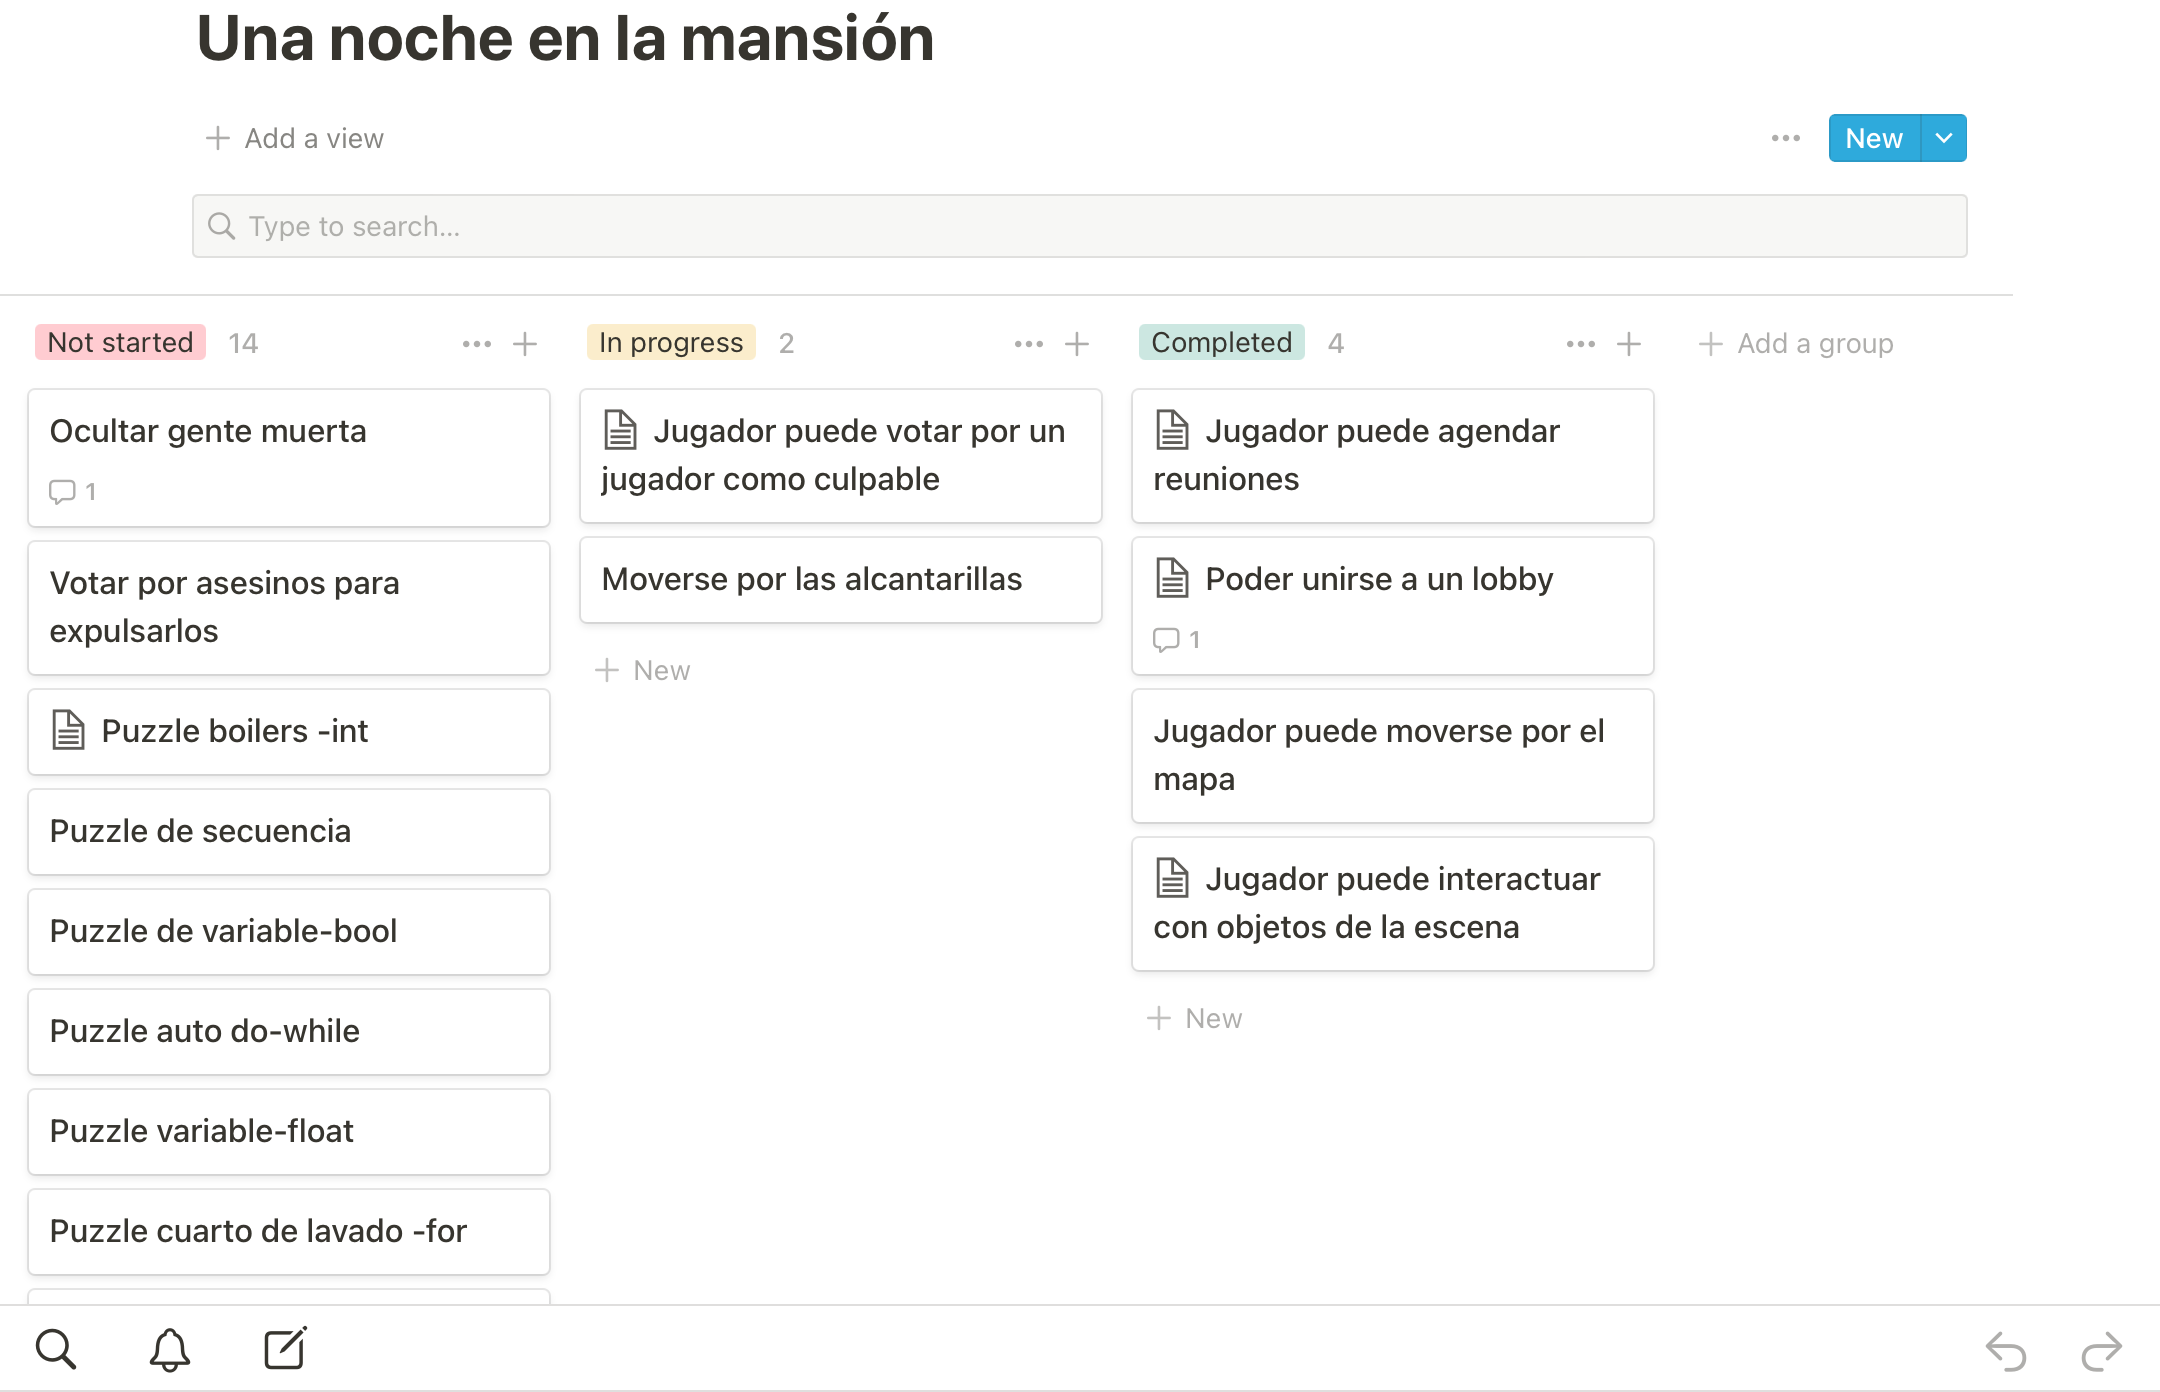
\includegraphics[width=0.8\linewidth]{images/notion.png}
    \caption{Notion con las actividades en diagrama \textit{Kanban}}
    \label{fig:notion_proyecto}
\end{figure}
\begin{figure}[H]
    \centering
    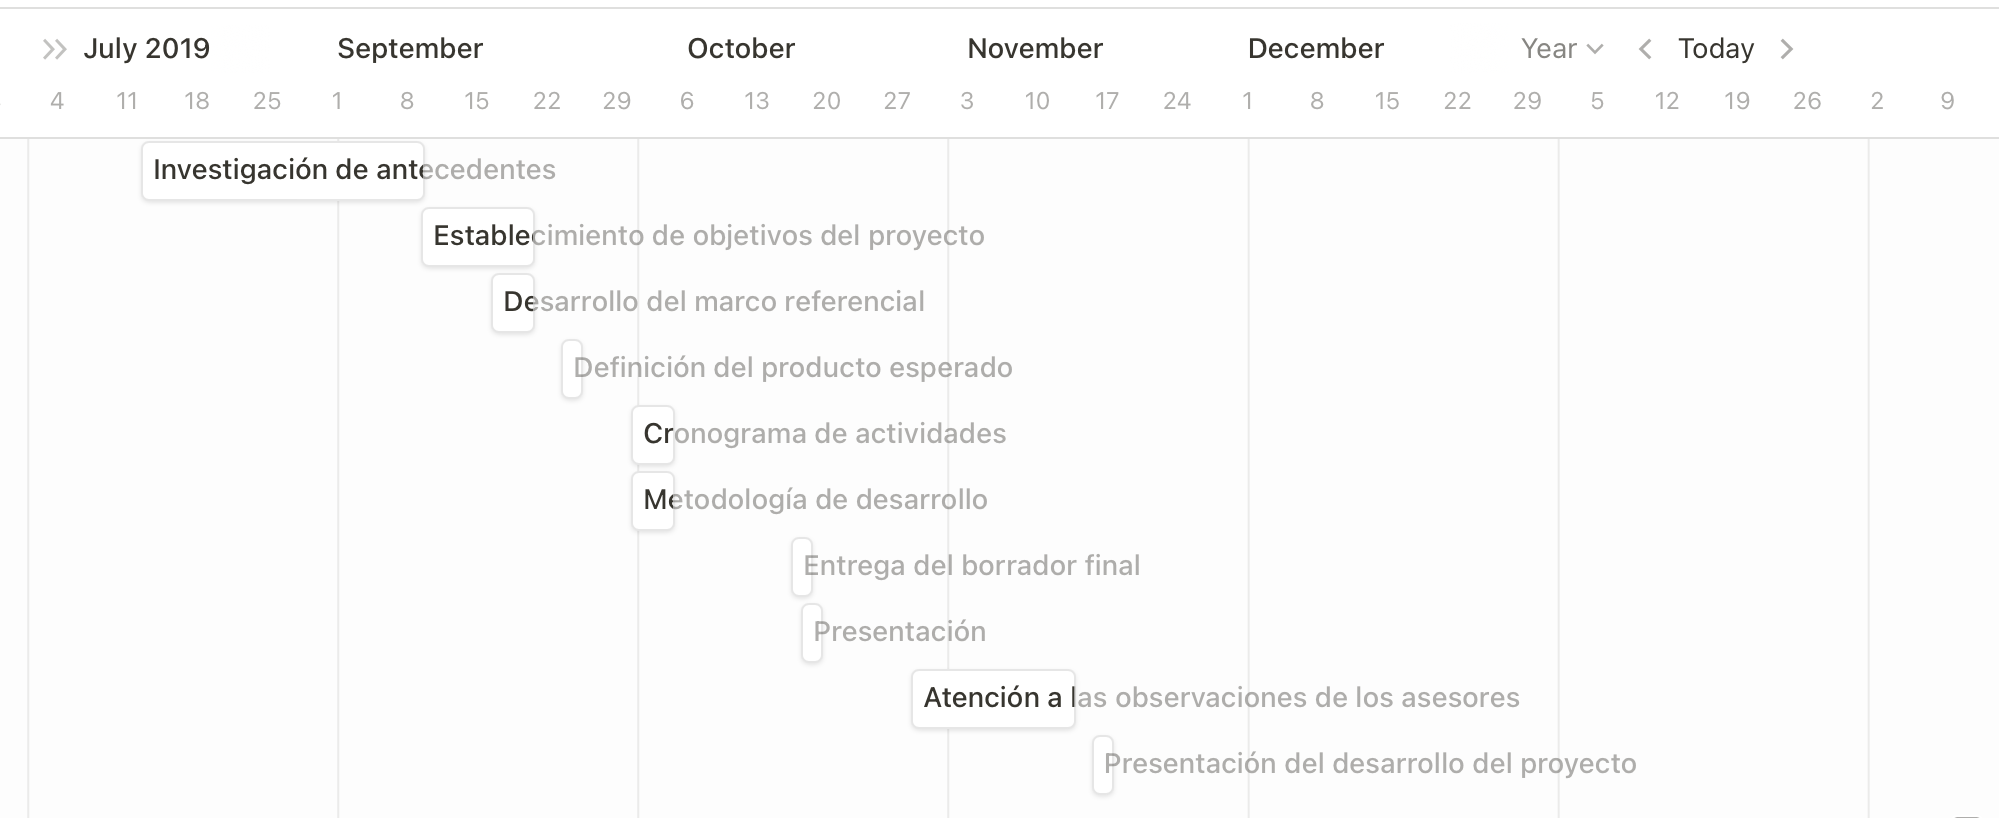
\includegraphics[width=0.8\linewidth]{images/DiagramaGanttAnteproyecto.PNG}
    \caption{Diagrama de Gantt del anteproyecto}
    \label{fig:gantt_anteproyecto}
\end{figure}
\begin{figure}[H]
    \centering
    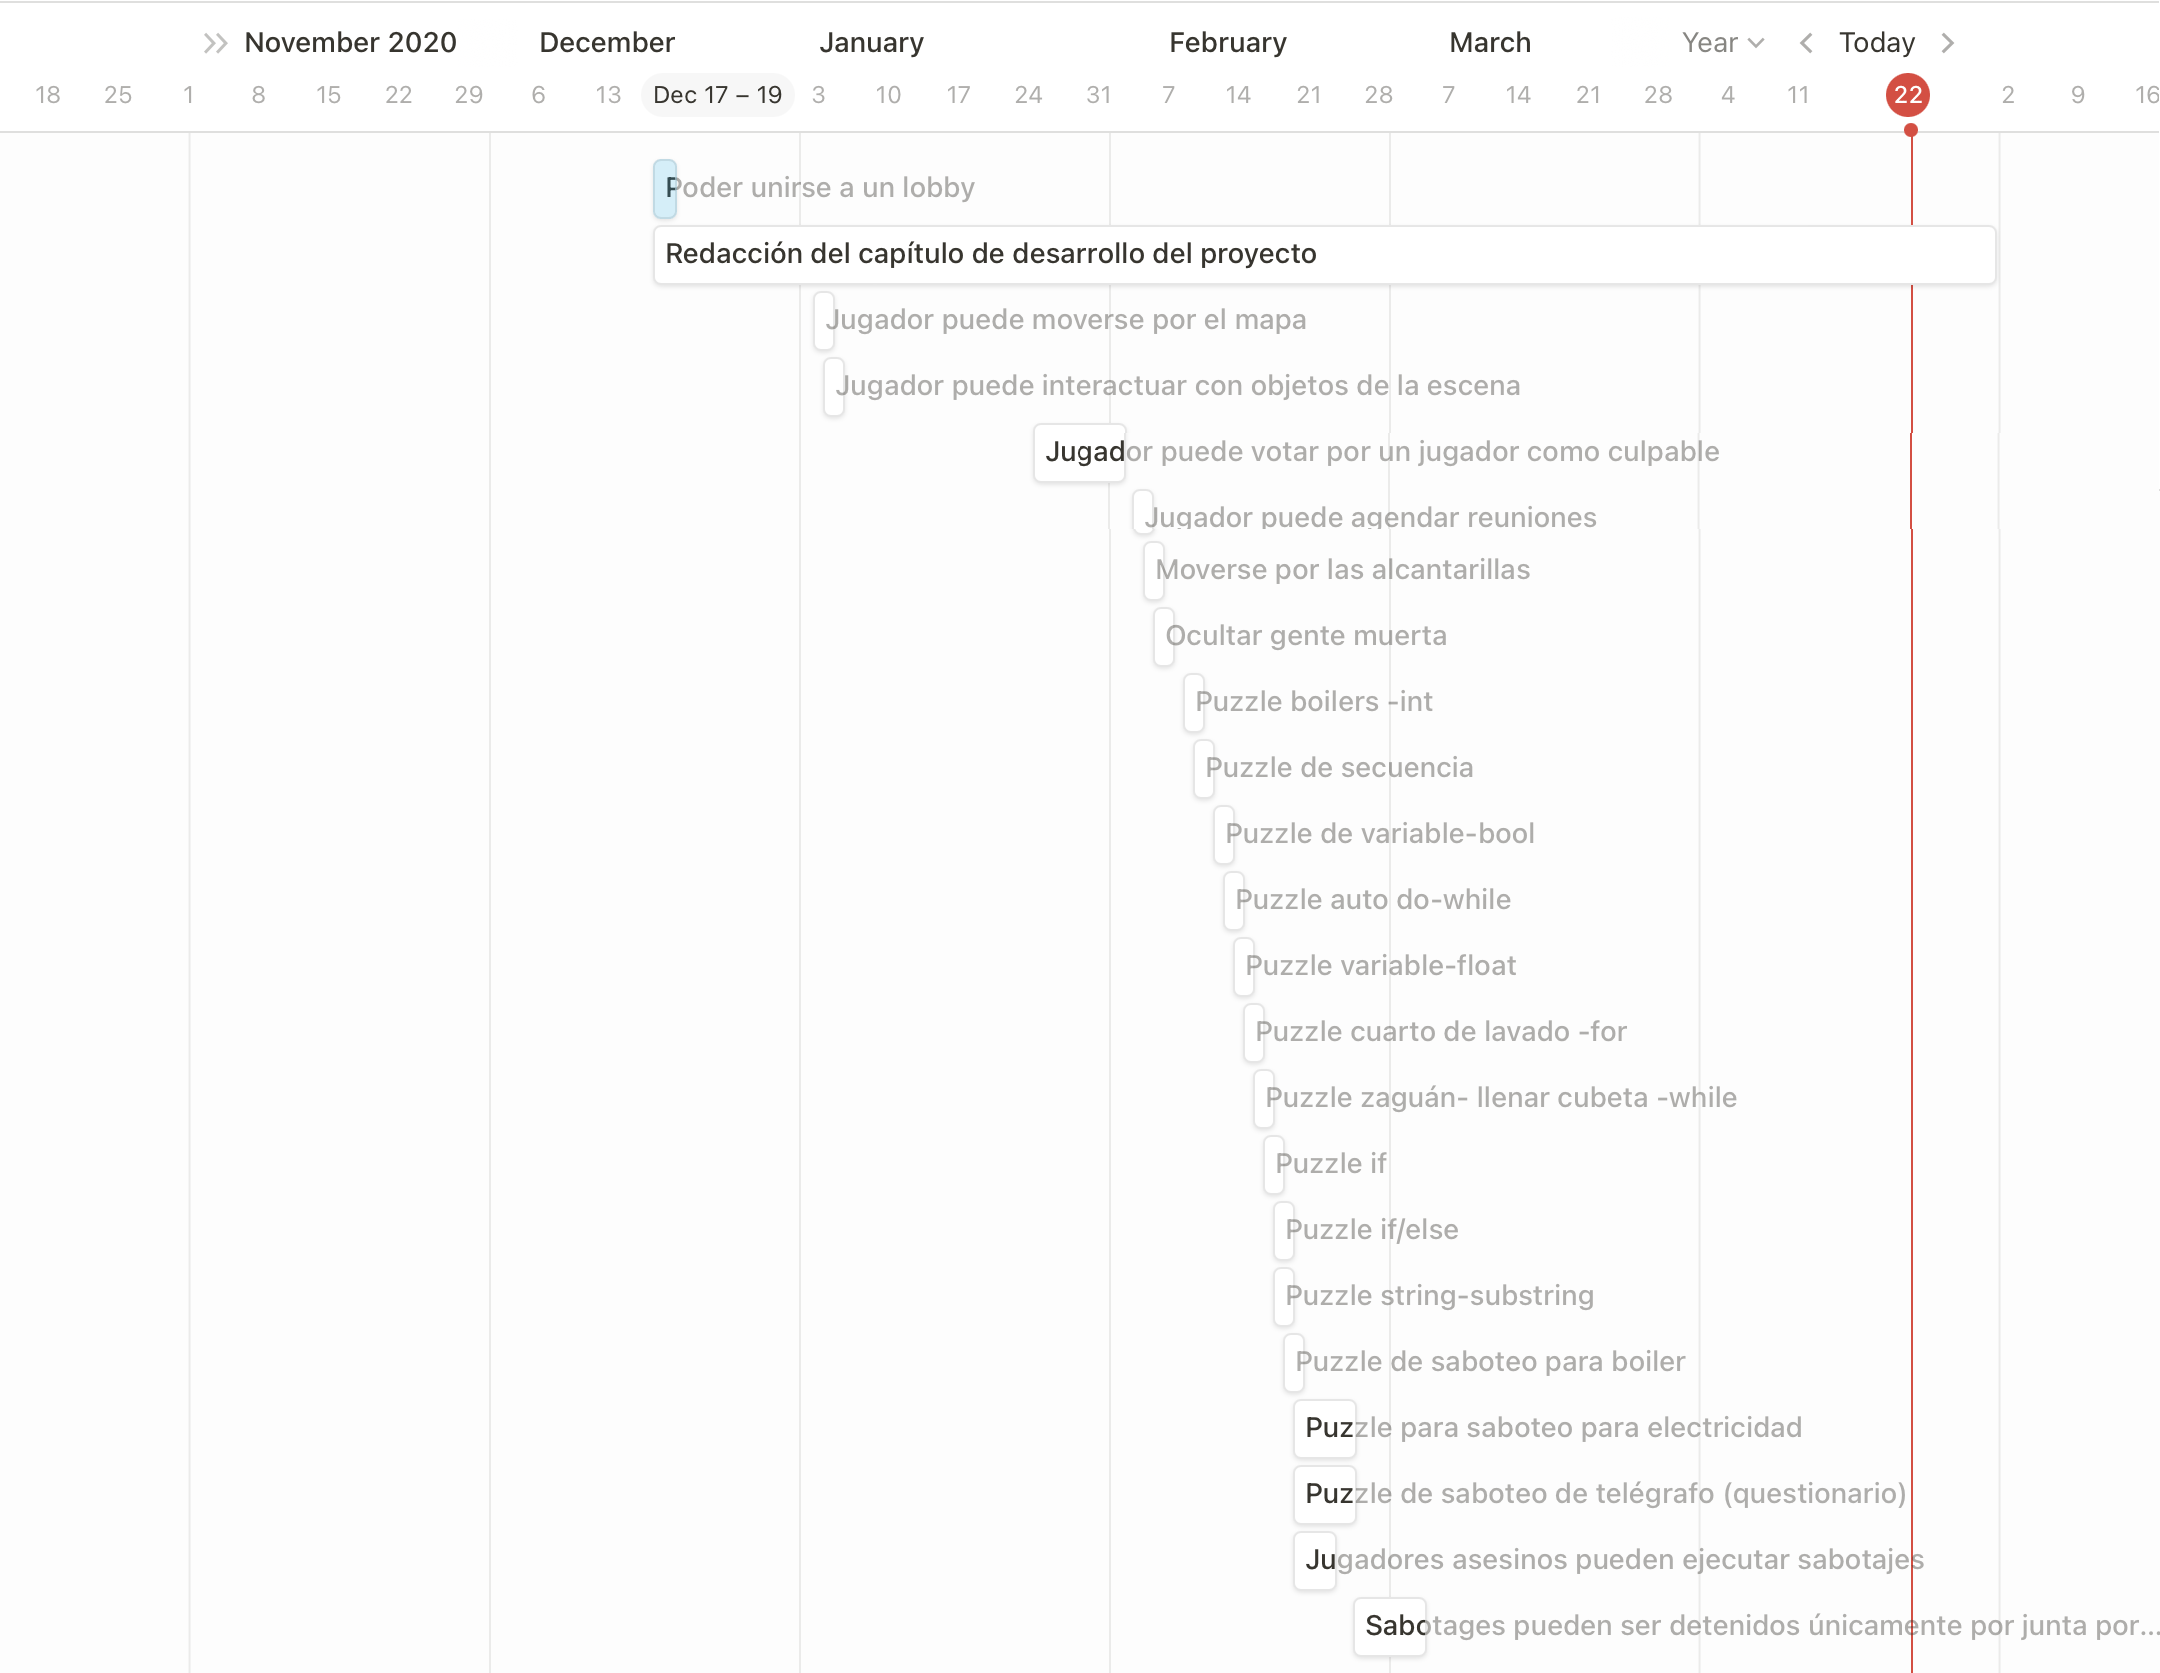
\includegraphics[width=0.8\linewidth]{images/MapaGanttProyecto.png}
    \caption{Diagrama de Gantt de la realización del proyecto}
    \label{fig:gantt_proyecto}
\end{figure}

\begin{figure}[H]
    \centering
    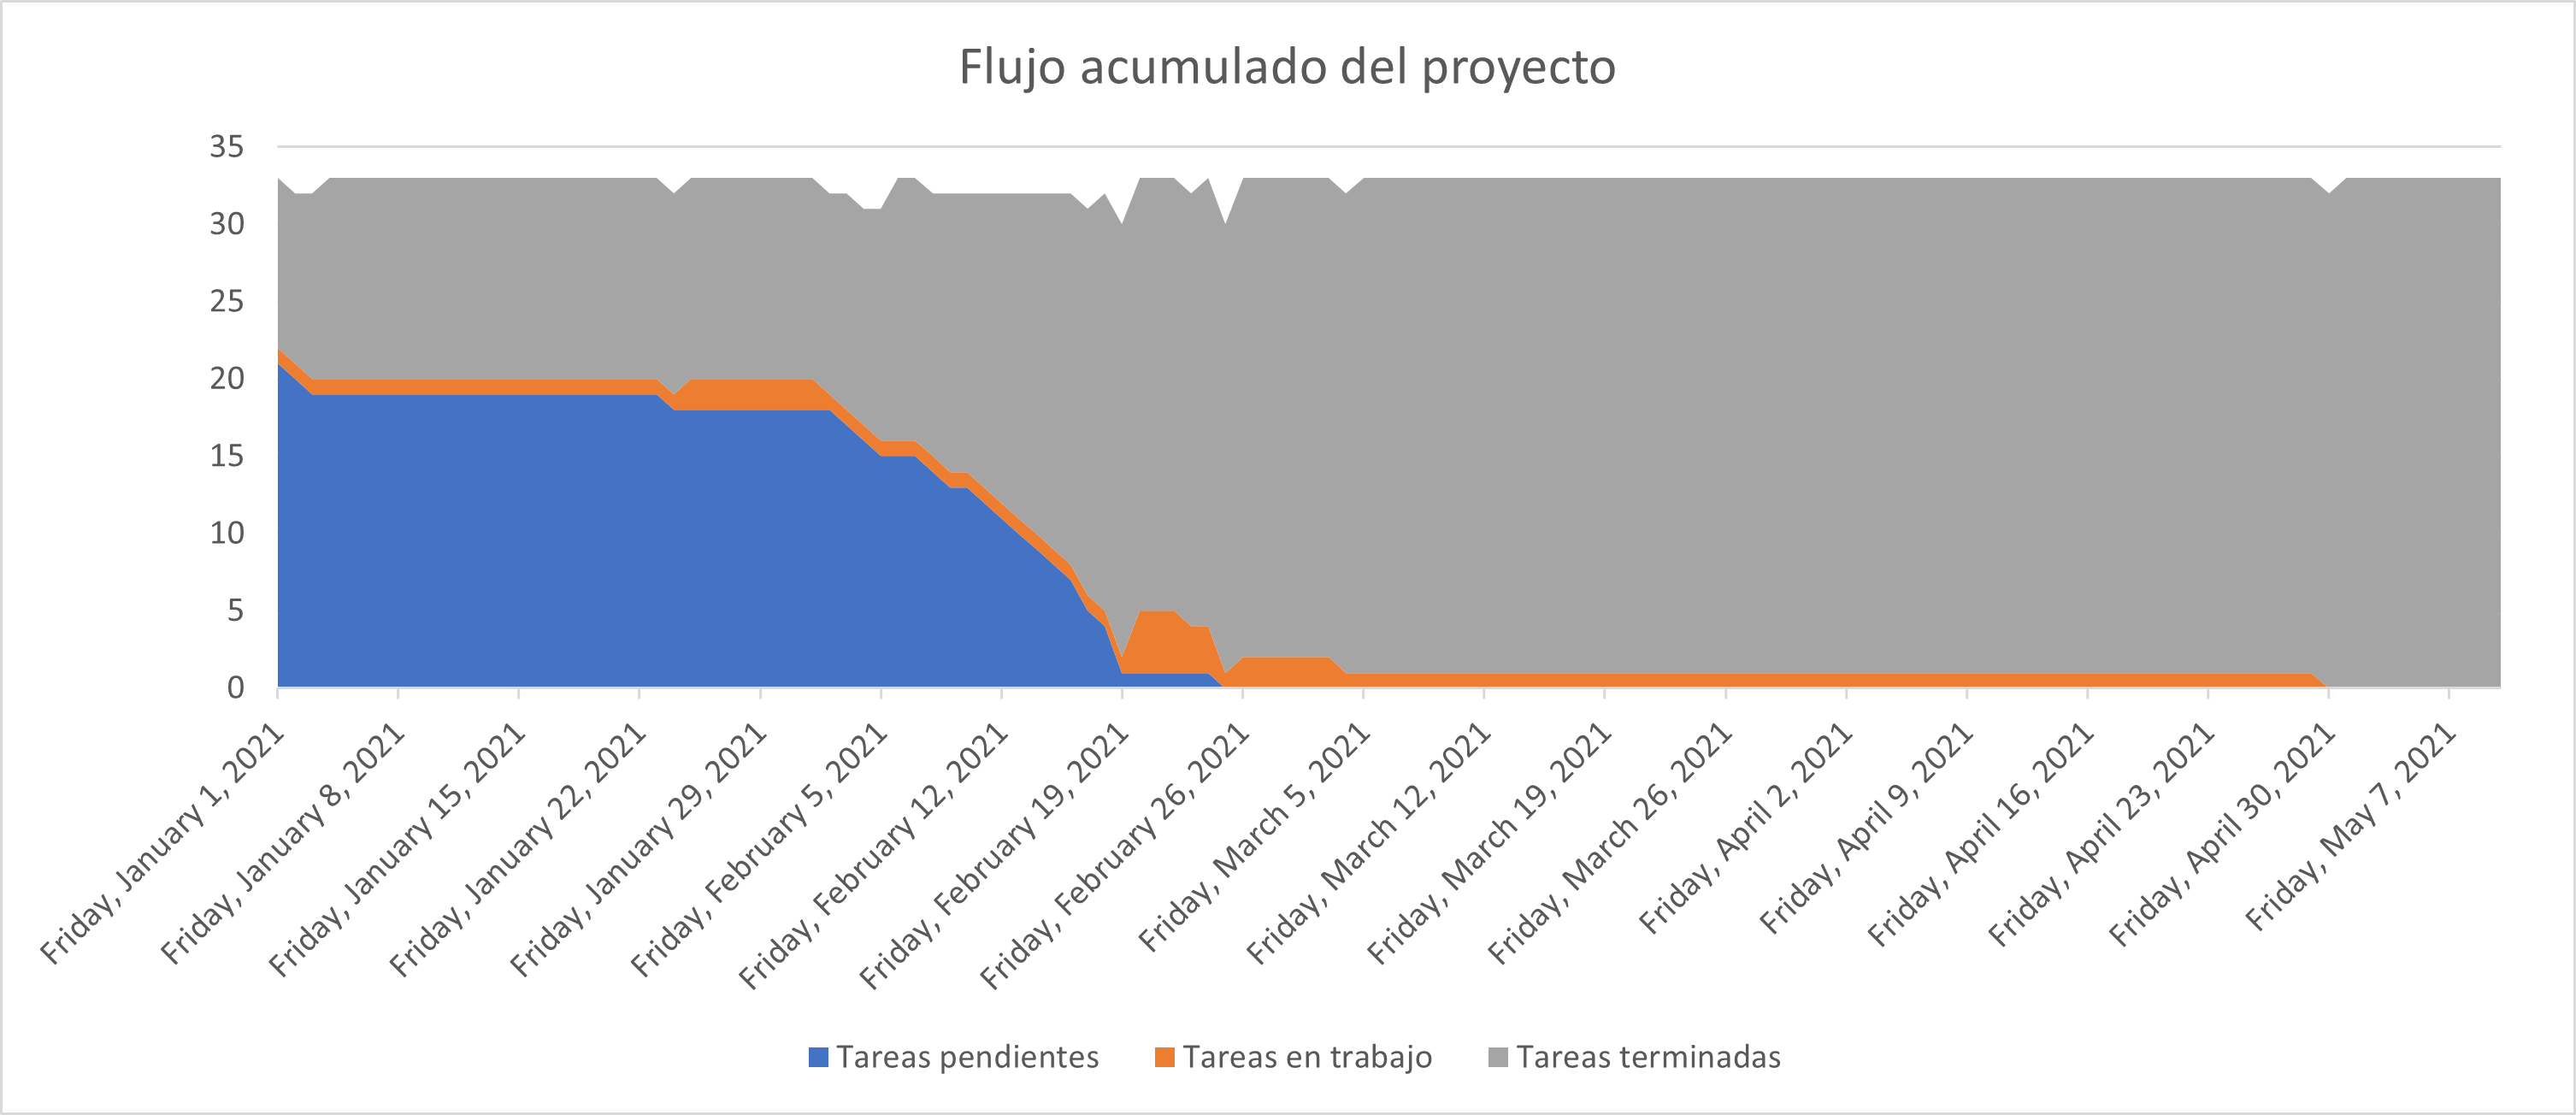
\includegraphics[width=0.8\linewidth]{images/BurndownChart.png}
    \caption{Gráfica de flujo acumulado del proyecto}
    \label{fig:grafica_flujo_acumulado}
\end{figure}
\begin{figure}[H]
    \centering
    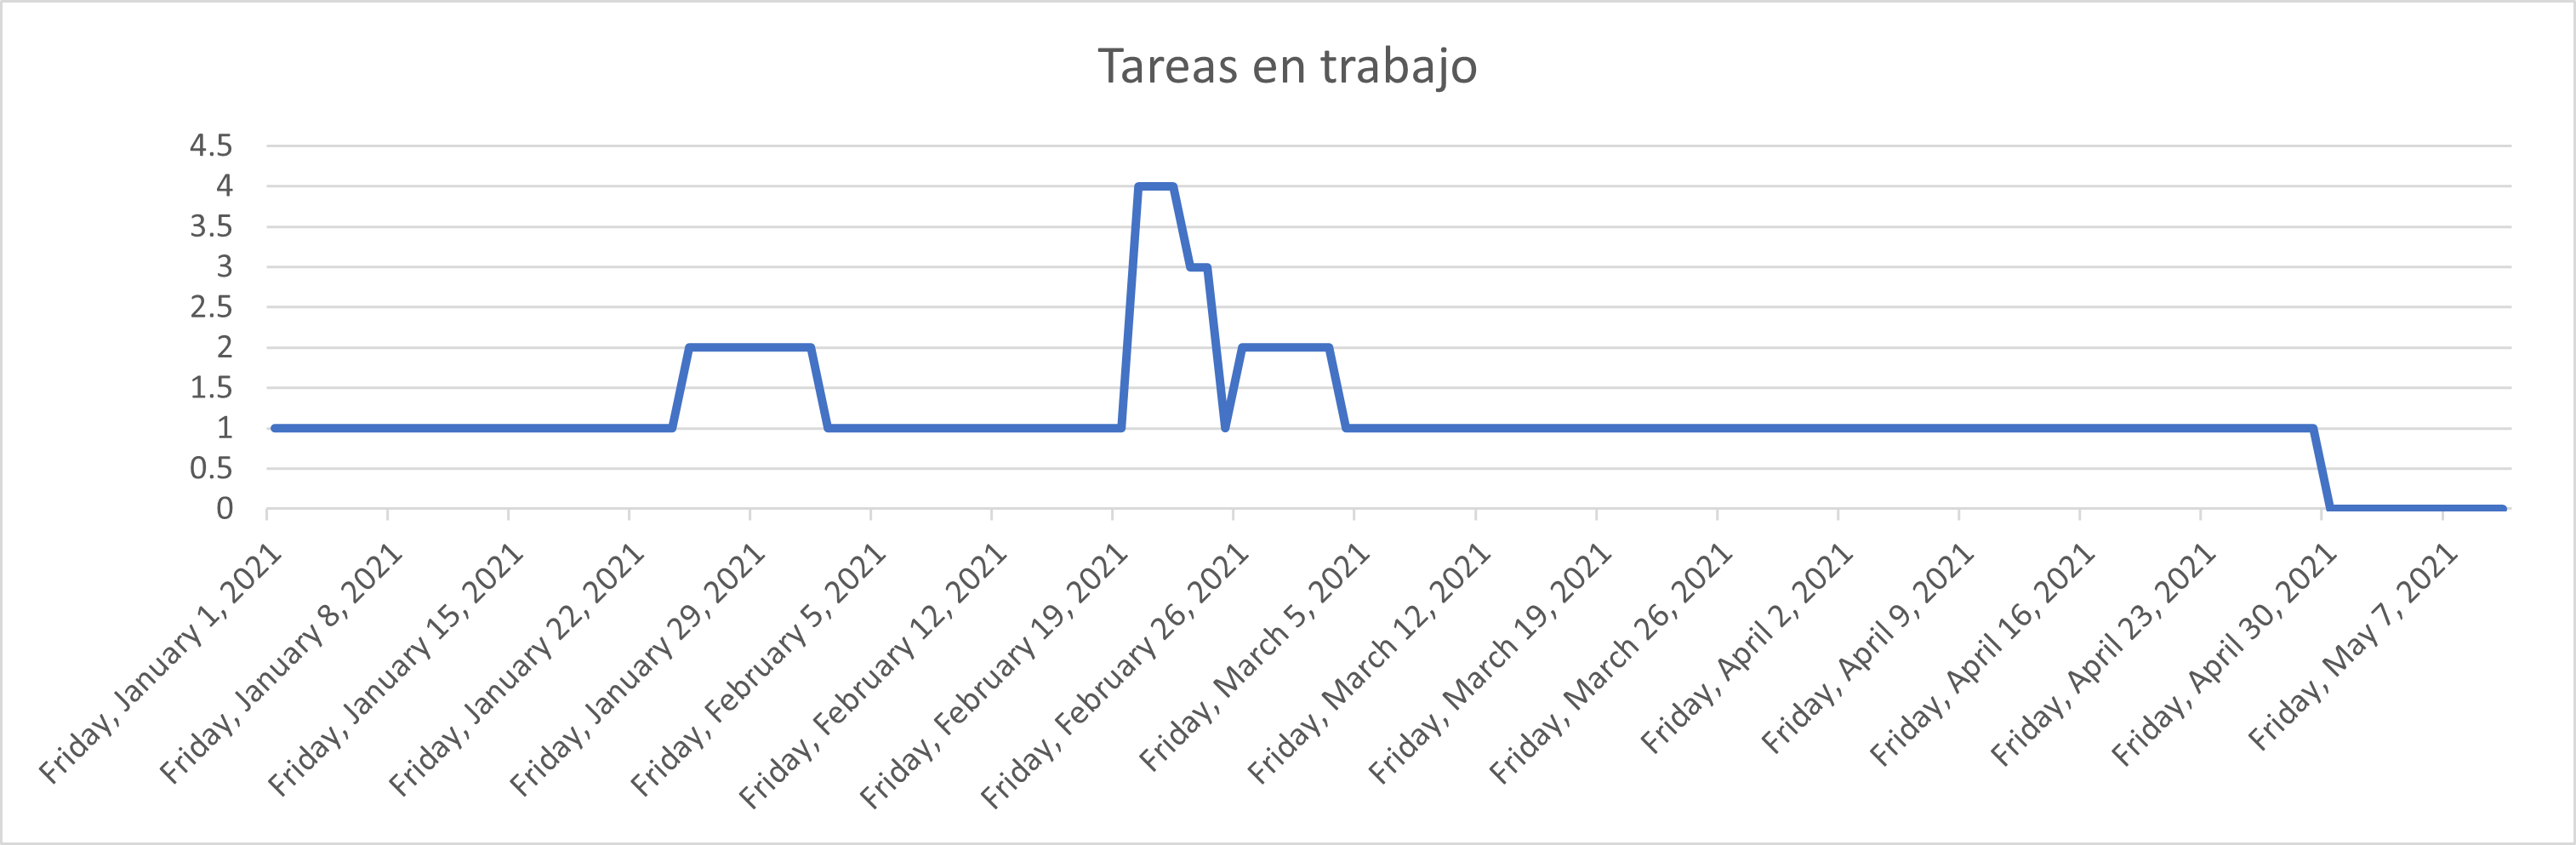
\includegraphics[width=0.8\linewidth]{images/TareasEnTrabajo.png}
    \caption{Gráfica de distribución de tiempos de ciclo del proyecto}
    \label{fig:grafica_tiempos_ciclo}
\end{figure}

\subsection{Análisis}
\subsubsection{Propuestas de producto}
Durante la definición del proyecto empezó la pandemia del SARS-COV2 que genera el padecimiento COVID-19. Ante la necesidad del aislamiento mucha gente recurrió a una gran variedad de juegos para ocupar su tiempo libre, entre estos hubo algunos juegos que ocuparon la consciencia colectiva por al menos un rato, juegos como \textit{Animal Crossing}, \textit{Fall Guys} y \textit{Among Us}. Muchos de estos juegos la gente los descubrió en \textit{streams}(transmitido en tiempo real) de gente jugando con sus amigos, estos normalmente jugaban el juego mientras estaban en videollamada. Un juego con ventajas similares que funcione tanto en un entorno en línea, así como en un salón de clases, tiene la utilidad como actividad integradora porque naturalmente hace que entre compañeros hablen y permite conocer a otras personas.
En su parte, se enfocó a que la creación del juego el usuario pueda aprender programación junto con sus compañeros incluso cuando estos no comparten un mismo espacio físico, dado que, durante la definición de este, muchos estudiantes tuvieron la necesidad de tomar clases a distancia. Ante esto, la preferencia que el juego fuera accesible en una multitud de dispositivos, a fin de que una gran variedad de estudiantes pueda acceder con su dispositivo o un dispositivo de la institución para participar en la actividad. Con este factor se consideró la necesidad de crear un juego para navegador como producto final. A base de la experiencia previa, así como sus plataformas soportadas y su facilidad para el desarrollo se decidió usar \textit{Unity} como \textit{game engine}.

\section{Diseño}
\subsection{Documento de diseño}
Se trabajó en un documento detallando los diferentes sistemas del juego. En este se definieron aspectos del juego como los diferentes puzzles como ejercicios de programación que tendrá que realizar el jugador para avanzar en el juego, el arte del juego, habitaciones, mecánicas, etc.

\subsubsection{Puzzles}
Los puzzles del juego fueron pensados para traer analogías del mundo real para explicar el funcionamiento de los diferentes conceptos a tratar. Con la limitante que el juego está orientado en Inglaterra en la tarde época victoriana, cuando invenciones como la electricidad empezaron a ganar fuerza.
Para cubrir los conceptos de programación estructurada se crearon los siguientes \textit{puzzles}:

\begin{itemize}
    \item Variables numéricas tipo enteras: Con un cuarto de \textit{boilers} en un extremo de la casa para brindar agua caliente, el jugador ajusta la temperatura a la que marca el termómetro, como se puede ver en la figura figura~\ref{fig:puzzle_int}. El \textit{puzzle} se completa si el usuario mueve el \textit{slider} a la temperatura correcta. Pensado en la vida real que los microcontroladores normalmente leen los valores de sensores.
    \begin{figure}[H]
        \centering
        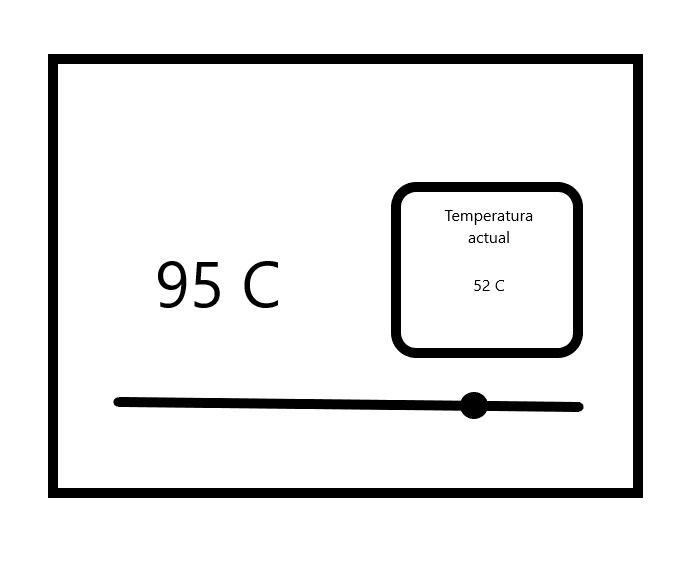
\includegraphics[width=0.5\linewidth]{images/PuzzleInt.png}
        \caption{Puzzle de variable numérica de tipo entero }
        \label{fig:puzzle_int}
    \end{figure}
    \item Secuencia: Entrena al jugador en su lógica de programación al trabajar en el jugador la habilidad de resolver problemas en paso. Requiere usar las teclas de dirección para moverse, requiere considerar el camino a tomar para llegar al otro lado. Cuenta como completado cuando el jugador se haya desplazado hasta el otro extremo de campo de juego del \textit{puzzle} (figura~\ref{fig:puzzle_secuencia}). Este \textit{puzzle} está pensado en que el jugador considere los pasos necesarios para llegar a la meta, lo necesario para la creación de algoritmos.
    \begin{figure}[H]
        \centering
        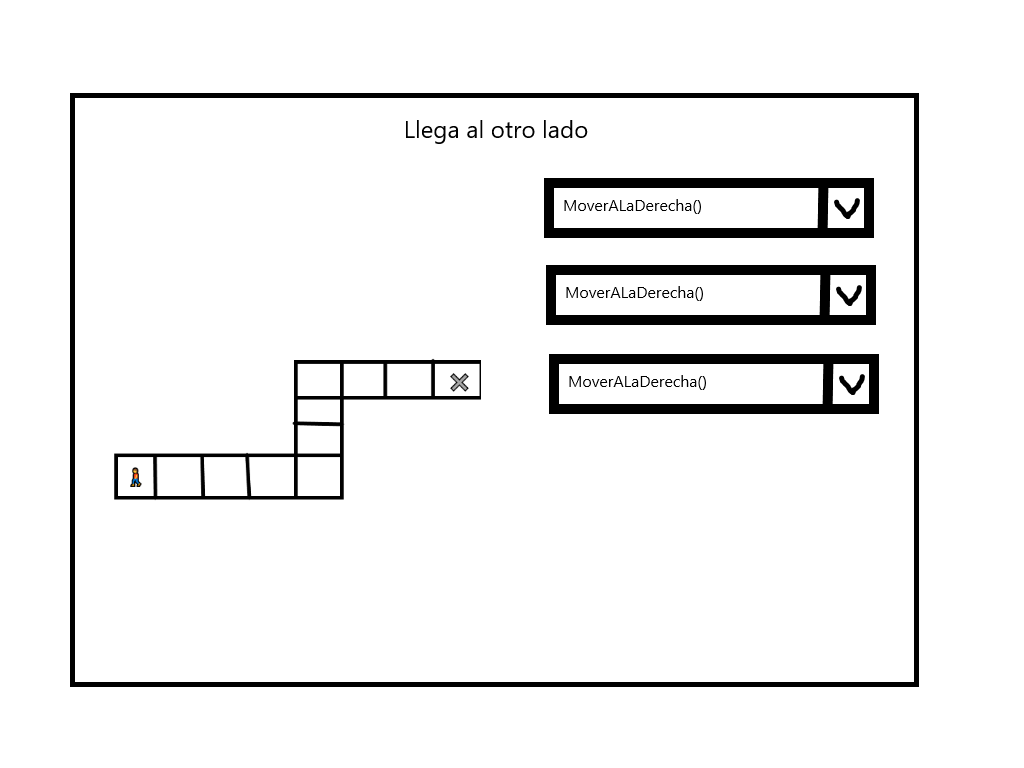
\includegraphics[width=0.5\linewidth]{images/PuzzleSecuencia.png}
        \caption{Puzzle de secuencia}
        \label{fig:puzzle_secuencia}
    \end{figure}
    \item Variables tipo string: El jugador teclea su nombre, al finalizar, un robot de servicio mostrara una burbuja de dialogo dándole la bienvenida (figura~\ref{fig:puzzle_string}). La motivación de este \textit{puzzle} es que normalmente las variables \textit{string} contienen información a imprimir en pantalla y requieren operaciones como concatenación para tenerla en el formato adecuado.
        \begin{figure}[H]
        \centering
        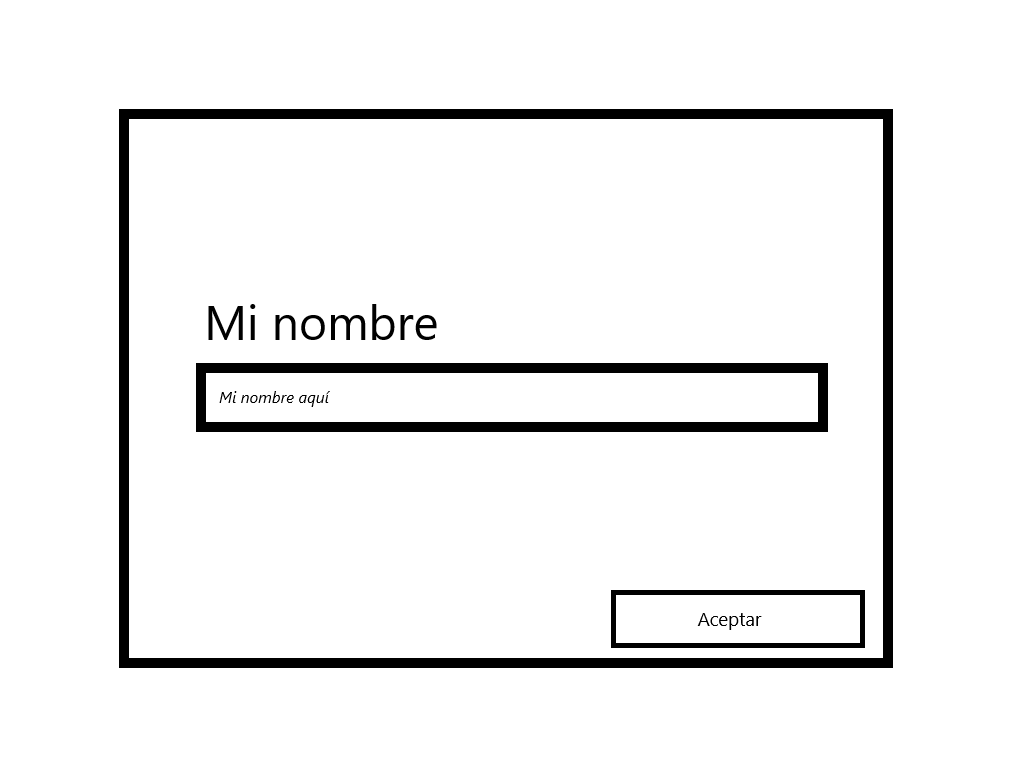
\includegraphics[width=0.5\linewidth]{images/PuzzleString.png}
        \caption{Puzzle de cadena de texto}
        \label{fig:puzzle_string}
    \end{figure}
    \item  Variables tipo booleano: Este tipo de variables son representadas como un \textit{switch} o un \textit{checkbox}. El jugador tendrá que volver a encender el generador moviendo la palanca. Un clic mueve la palanca de una posición a la siguiente y completa el \text{puzzle}, como se ve en la figura~\ref{fig:puzzle_booleano}. Pensada en el uso de los booleanos como banderas, para indicar el estado de un objeto. 
    \begin{figure}[H]
        \centering
        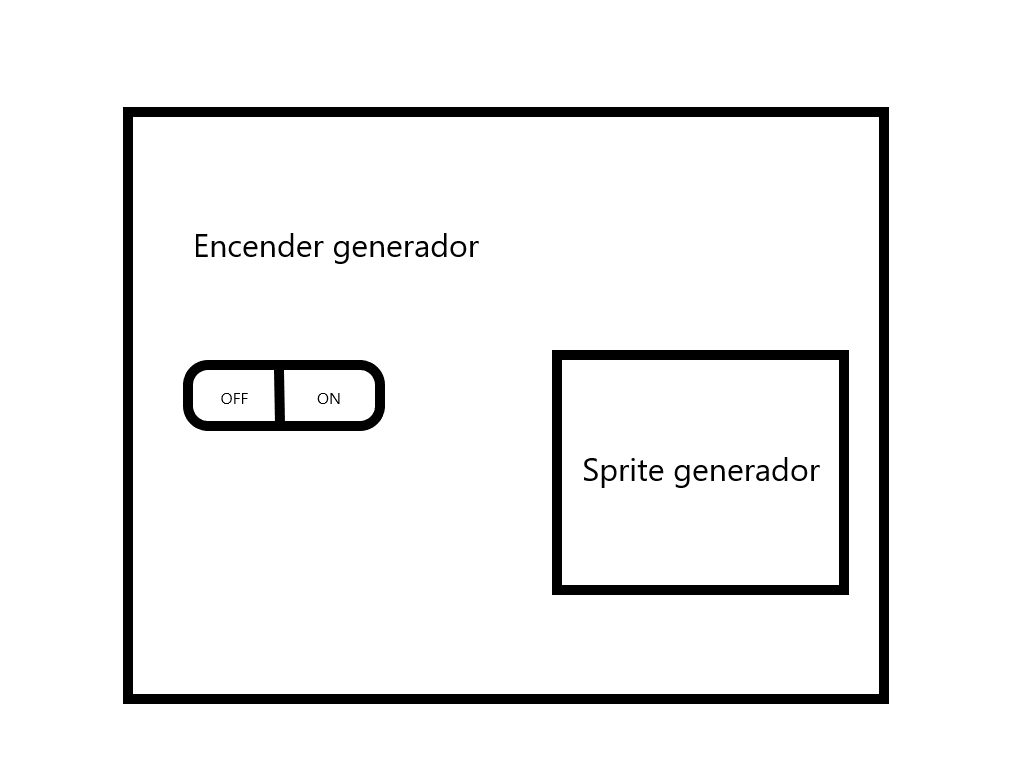
\includegraphics[width=0.5\linewidth]{images/SabotageGenerador.png}
        \caption{Puzzle de secuencia}
        \label{fig:puzzle_booleano}
    \end{figure}
    \item Do While: Un \textit{do while} es útil cuando la tarea a realizar requiere hacer algo al menos una vez, en este caso usamos la palanca de arranque de un automóvil que puede requerir una vuelta o unas cuantas y cuando se inicia, se tiene que alejar la mano o en la vida real uno se puede lesionar por la fuerza del motor. El usuario completa el puzzle de manera que se intente arrancar el motor siempre que no haya encendido, el jugador entra el valor booleano que funcione el código de la manera correcta, la interfaz gráfica que mostrara se puede ver en la figura~\ref{fig:puzzle_do_while}.
    \begin{figure}[H]
        \centering
        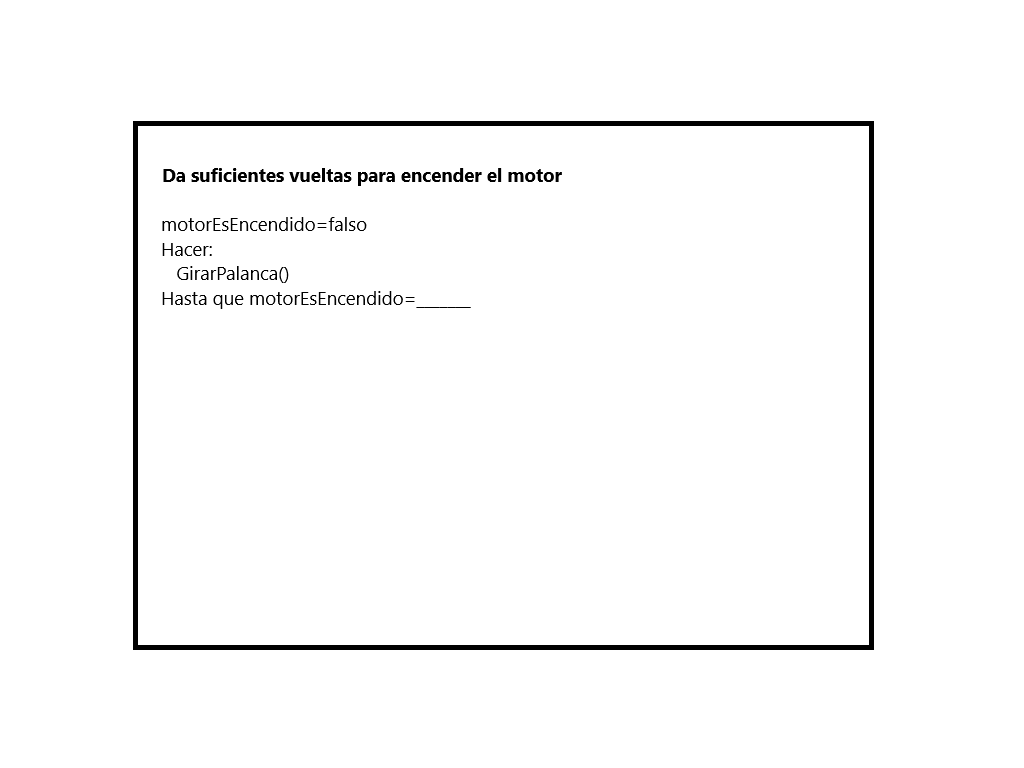
\includegraphics[width=0.5\linewidth]{images/PuzzleDoWhile.png}
        \caption{Puzzle de estructura do while}
        \label{fig:puzzle_do_while}
    \end{figure}
    \item Variable numérica de punto flotante: Un \textit{puzzle} más avanzado que el de variable tipo entero, como se ve en la figura~\ref{fig:puzzle_float} el jugador introduce la temperaturas, por experiencia de usuario se cambia el \textit{slider} a una caja donde el jugador tendrá que teclear el valor actual de la temperatura.
    \begin{figure}[H]
        \centering
        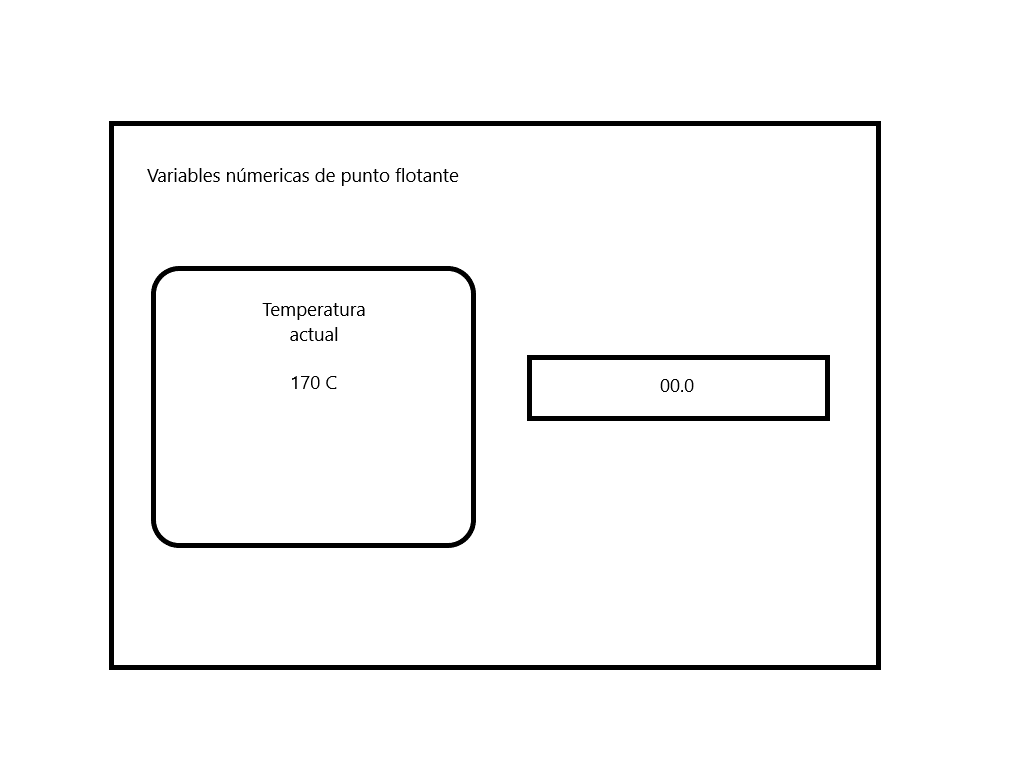
\includegraphics[width=0.5\linewidth]{images/PuzzleFloat.png}
        \caption{Puzzle de variable float}
        \label{fig:puzzle_float}
    \end{figure}
    \item Ciclo tipo for:Se asemeja al ciclo de una lavadora que dura cierta duración, el jugador necesita que poner las veces que la lavadora da vuelta la ropa (figura~\ref{fig:puzzle_for}).
    \begin{figure}[H]
        \centering
        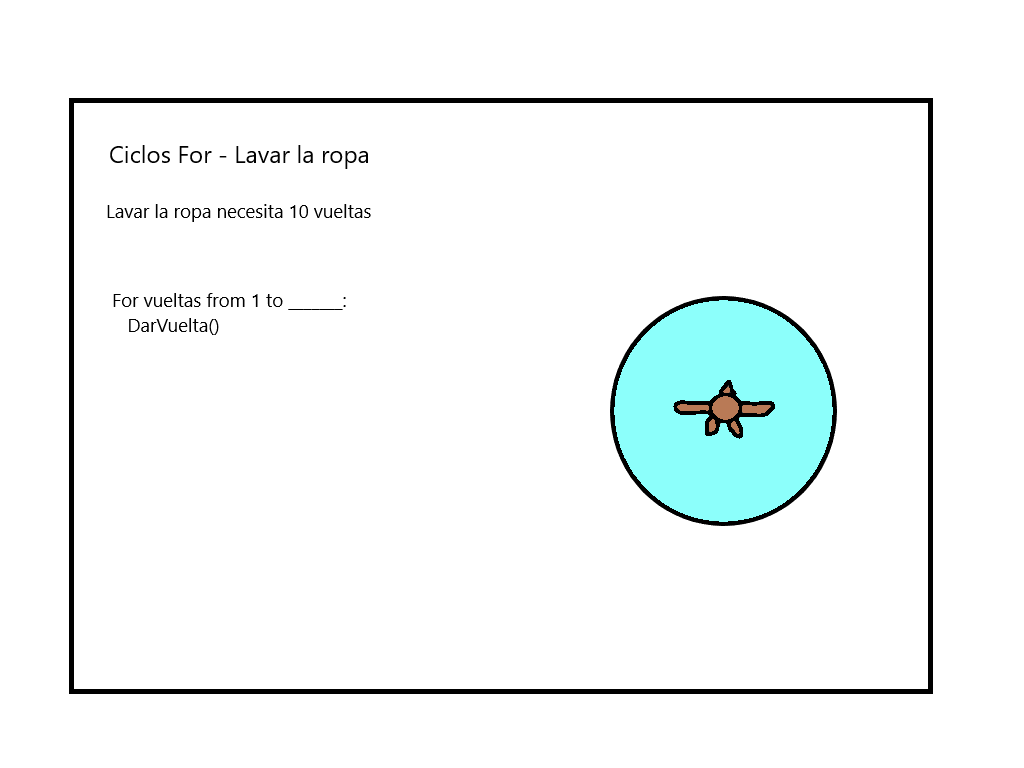
\includegraphics[width=0.5\linewidth]{images/PuzzleFor.png}
        \caption{Puzzle de estructura for}
        \label{fig:puzzle_for}
    \end{figure}
    \item Ciclo tipo while: Una cubeta requiere cierta cantidad de agua para llenarla hasta cierto punto, o si no, se tira el agua de la cubeta (figura~\ref{fig:while_puzzle}). Este concepto permite realizar una acción monitoreando mediante una condición el nivel de la cubeta y así detenerse, algo así como el uso de la estructura \textit{while} para la lectura del contenido de un archivo por poner un ejemplo.
        \begin{figure}[H]
            \centering
            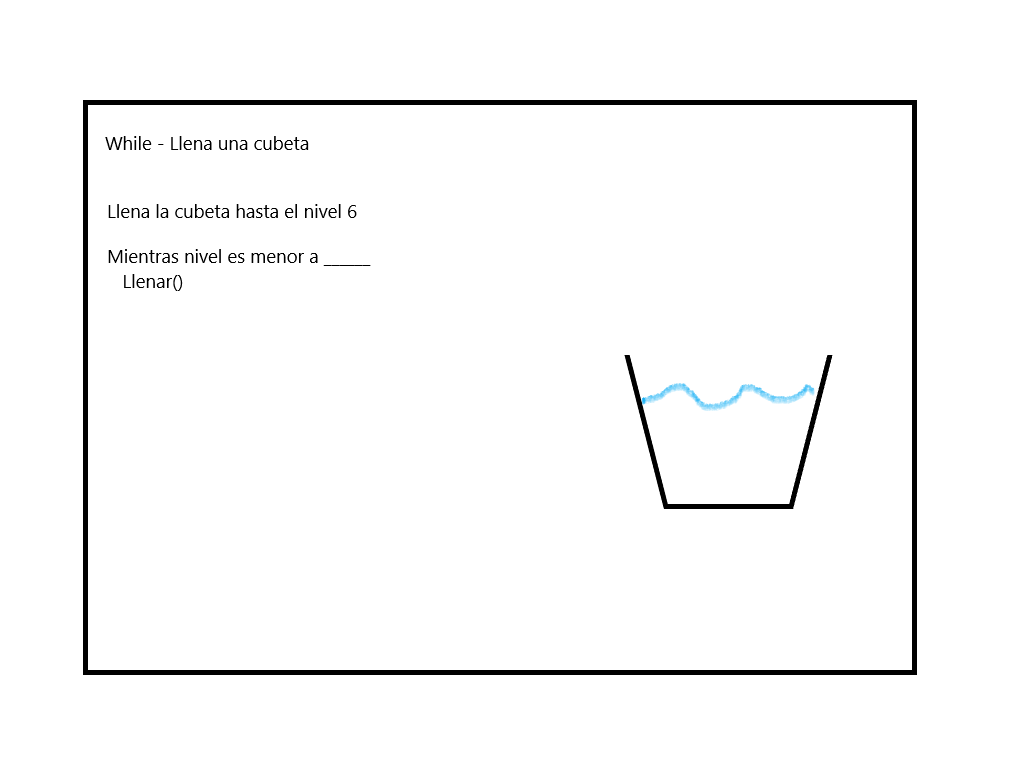
\includegraphics[width=0.5\linewidth]{images/WhilePuzzle.png}
            \caption{Puzzle de while}
            \label{fig:while_puzzle}
        \end{figure}
    \item Condicional simple: Los jugadores tendrán que seleccionar la flor del tipo correcto a poner en el florero, como se nota en la figura~\ref{fig:puzzle_if}. La forma en la que los usuarios saben cuál es la solución correcta es por un pseudocódigo que incluye un único \textit{if}, los usuarios tendrán que analizarlo para saber que flor \textit{tendrán} que seleccionar.
    \begin{figure}[H]
        \centering
        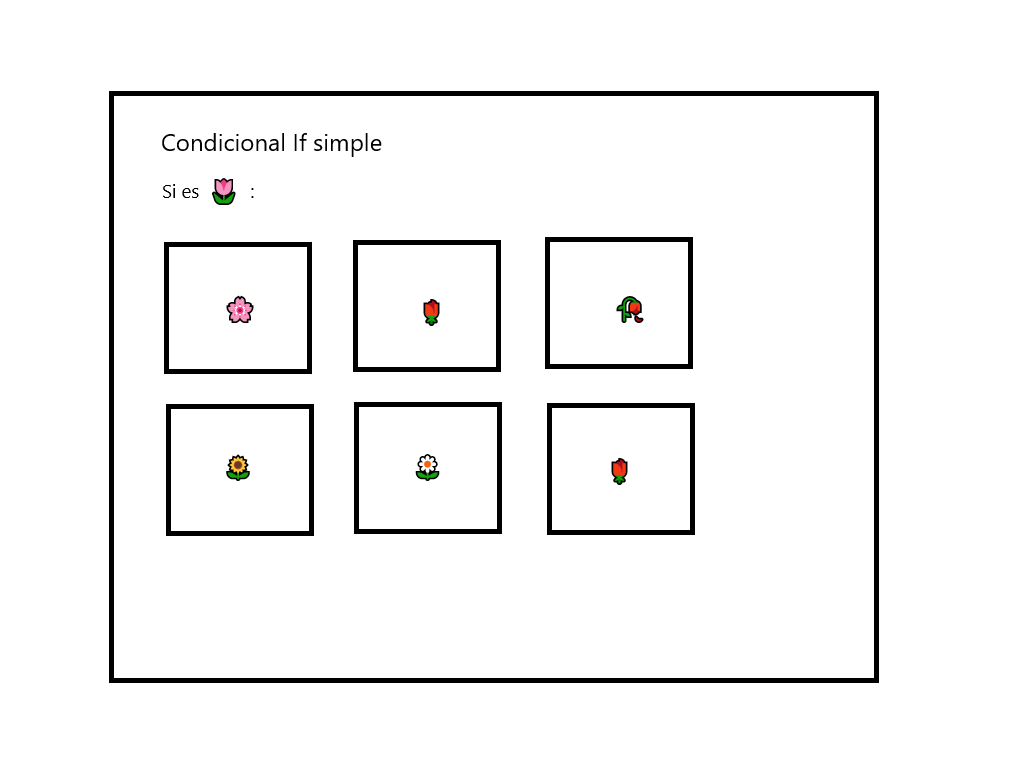
\includegraphics[width=0.5\linewidth]{images/PuzzleIf.png}
        \caption{Puzzle de seleccionar flor, usa selección para enseñar el uso del if}
        \label{fig:puzzle_if}
    \end{figure}
    \item Condicional con \textit{else}: Una versión extendida del \textit{if}. Haciendo alusión a la figura~\ref{fig:if_else_puzzle}, este consiste en decoración de repostería, en ese día se prepararon \textit{cupcakes} y pasteles,  el jugador será presentado el pseudocódigo de cual debería ser su decisión según el tipo de repostería. Las opciones serán mostradas como botones.
        \begin{figure}[H]
            \centering
            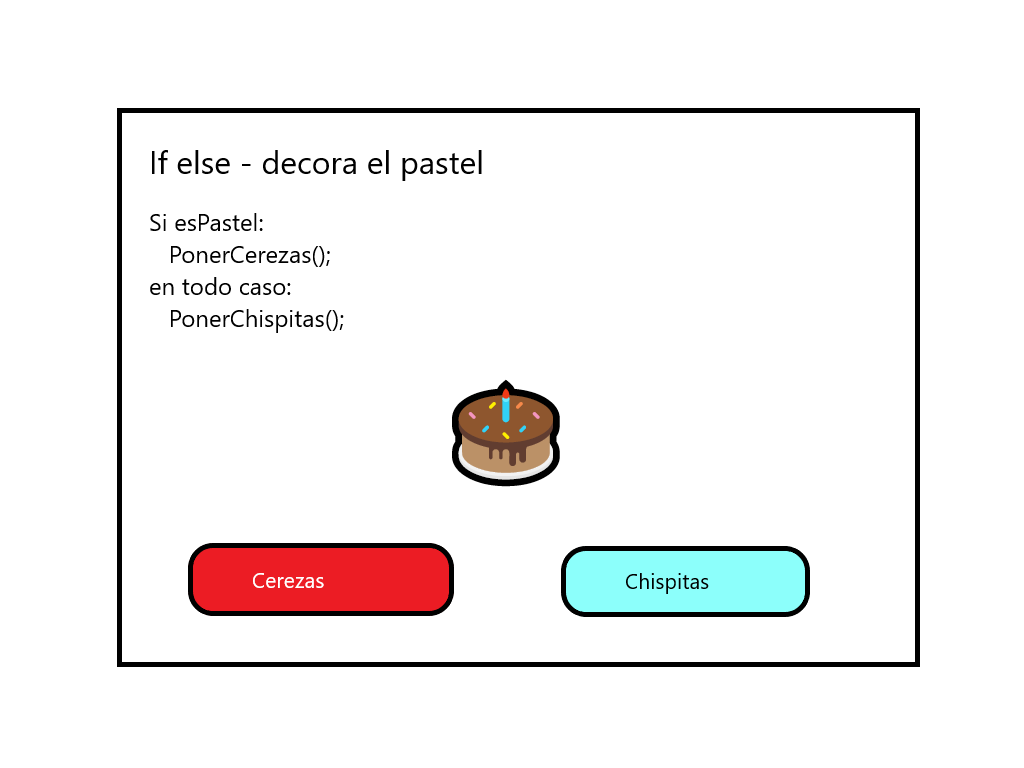
\includegraphics[width=0.5\linewidth]{images/PuzzleIfElse.png}
            \caption{Puzzle diseñado para el if/else}
            \label{fig:if_else_puzzle}
        \end{figure}
\end{itemize}

La organización de los puzzles se puede ver la figura~\ref{fig:items_on_map}. La mayoría de los puzzles están organizados dependiendo en su temática, por ejemplo: decoración de pasteles ocurre en la cocina. Sin embargo, se tomaron a la hora del diseño libertades para hacer que cuartos sean más justos, hay puzzles que su posición fue definida para crear un flujo de jugadores en ese cuarto, a forma de que haya lugares donde los asesinos pueden ir varias veces a encontrar jugadores programadores y a la vez evitar que si los agarran en estos lugares nadie se dé cuenta.
Los \textit{puzzles} se pueden descubrir por un símbolo de espada (figura~\ref{fig:puzzle_location}), los jugadores se tienen que parar cerca para interactuar con ellos, eso abre la interfaz gráfica para resolver los puzzles. Cuando estos no hayan sido resueltos tienen un icono, cuando ya fueron resueltos por un jugador este desaparece y no se puede interactuar con ellos.

\begin{figure}[H]
    \centering
    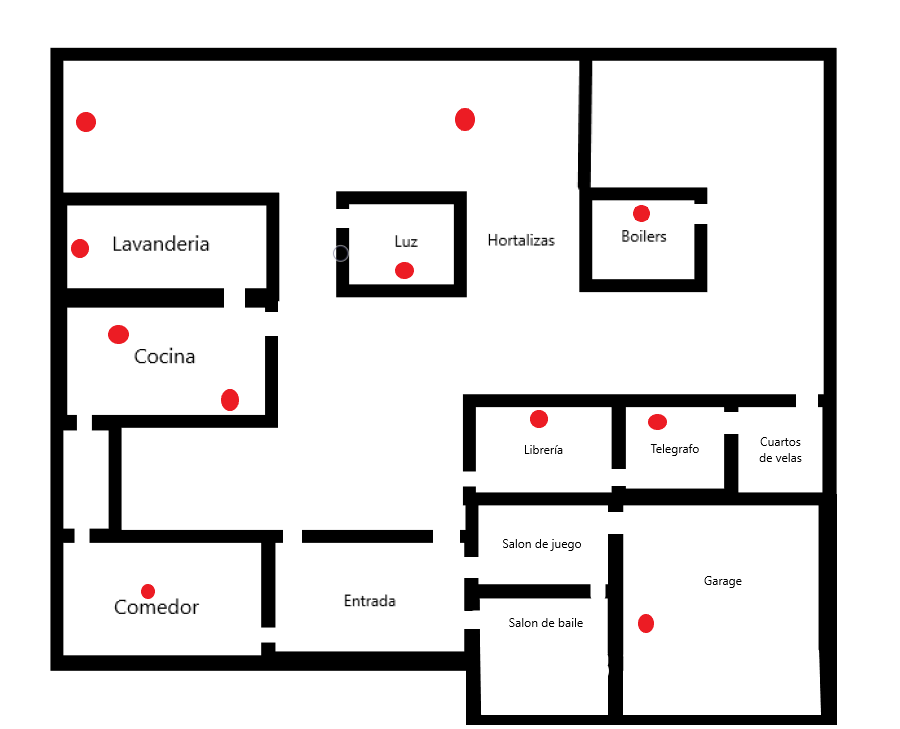
\includegraphics[width=0.5\linewidth]{images/MapaJuegoConItems.png}
    \caption{Disposición de \textit{puzzles} en el juego}
    \label{fig:items_on_map}
\end{figure}

\begin{figure}[H]
    \centering
    
\includegraphics[scale=0.5]{images/espada_sprite.png}
    \caption{\textit{Sprite} que indica que en ese lugar del juego es un \textit{puzzle}}
    \label{fig:puzzle_location}
\end{figure}

\begin{figure}[H]
    \centering
    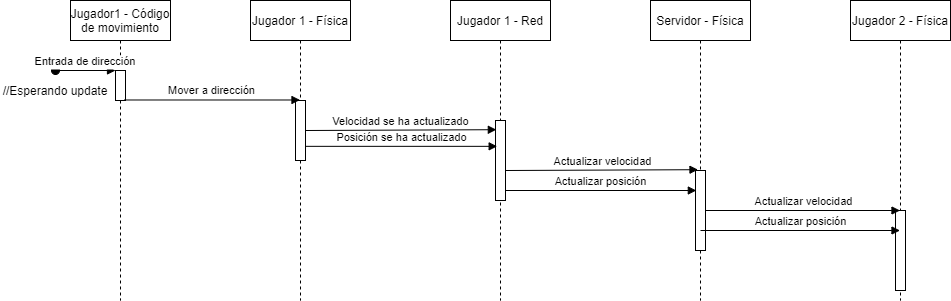
\includegraphics[width=1\linewidth]{images/diagrama_secuencia_movimientos.png}
    \caption{Diagrama de secuencia de los controles del jugador}
    \label{fig:diagrama_sec_movimiento}
\end{figure}

Se decidió utilizar la librería \textit{Mirror} para desarrollar el sistema de multijugador. Esto es esencial, porque sus abstracciones para el manejo de las comunicaciones cliente-servidor mediante \textit{Remote Call Procedure} dictaron algunas decisiones de arquitectura.
Este fue diseñado con un servidor autoritativo. Las acciones del jugador van al servidor para ser verificadas. Una excepción es el sistema de movimiento de los jugadores, como trataremos a continuación. Como se puede ver en la figura~\ref{fig:diagrama_sec_movimiento}, en este caso cada "propietario" de su personaje tiene capacidad total de moverlo a donde quiera, en teoría. En práctica, el cliente controla la posición a base de la entrada del jugador y usando sincronización de posición y velocidad de Mirror tenemos un pseudo sistema de predicción de su siguiente movimiento para conexiones lentas. 

\subsubsection{Sistema de detección de muertes}
Es un sistema que funciona primordialmente en el servidor, se puede notar su funcionamiento en la figura~\ref{fig:diagrama_sec_detect_muertes}. En todo momento, cada \textit{game loop} corre una rutina que realiza \textit{raytracing} al área circundante al jugador con un radio definido previamente en el \textit{lobby} del juego. Al haber un cambio se mandará una llamada a un procedimiento en el cliente que actualizará la interfaz gráfica para mostrar un botón de reportar muertos. Una vez al ser reportado, se realizará una segunda revisión de que sea una operación legal y se pide a todos los clientes mostrar una UI para realizar la votación sobre el personaje de juego.
\begin{figure}[h!]
    \centering
    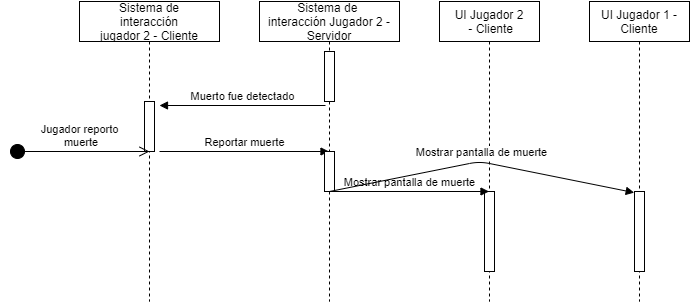
\includegraphics[width=1\linewidth]{images/diagrama_deteccion_muerte.png}
    \caption{Diagrama de secuencia de la detección de muertes}
    \label{fig:diagrama_sec_detect_muertes}
\end{figure}

\subsubsection{Asesinatos}
Hay un tipo de jugadores especiales llamados asesinos, estos son impostores que engañan a los demás jugadores de su verdadera identidad. Estos tienen entre una de sus capacidades matar a otros jugadores. El asesinar a otros jugadores es una actividad que solo el servidor tiene autoridad.
Como se nota en la figura~\ref{fig:diagrama_sec_muertes_por_impost}, se detectan los jugadores en el servidor. En el cliente del jugador impostor se puede matar a otros jugadores no impostores, cuando se manda la señal de matar a alguien (invocada por un botón) se pregunta al servidor si es legal o sea si es físicamente posible su ocurrencia (cercanía, no hay \textit{cooldown}, entre otros). Si es legal (si en ese momento puede matar a otro jugador), se llama el \textit{spawn} de una tumba en el lugar del jugador muerto y para mandarlo a otro \textit{layer} que no es visible a los jugadores vivos y mostrar la capa de fantasmas en la cámara del cliente para el jugador muerto mediante una función RPC. En el caso de los demás jugadores solo recibirán por parte del servidor un mensaje para \textit{spawnear} una tumba y desaparecerá ese jugador de su juego.
\begin{figure}[h!]
    \centering
    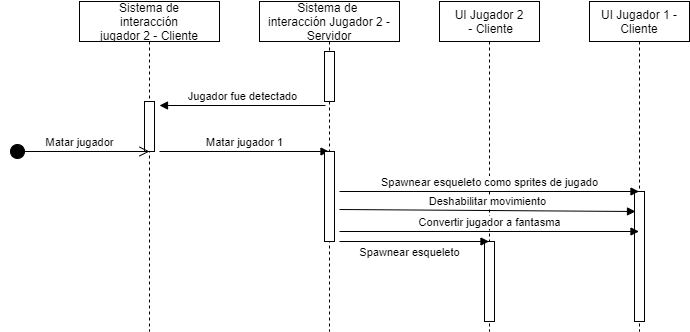
\includegraphics[width=1\linewidth]{images/diagrama_sec_matar.png}
    \caption{Diagrama de secuencia de muertes por asesinos/impostores}
    \label{fig:diagrama_sec_muertes_por_impost}
\end{figure}

\subsubsection{Votación de asesinos}
La votación se puede invocar de dos formas distintas; la primera forma es cuando algún jugador (ya sea programador o asesino) reporta que encontró una tumba y la segunda es acudiendo a el botón de emergencia ubicado cerca del punto donde los jugadores inician la partida. Cuando la votación se muestra una UI que permite votar por quien es el impostor (figura~\ref{fig:diagrama_ui_votacion}). En esta parte, los jugadores pueden hablar (en su salón de clases, en videollamada o \textit{chat} de voz usando una aplicación externa) para llegar a un acuerdo por quién votar, puede compartir información o pistas que encontraron durante su partida, decir que tareas tuvieron antes de la votación, etc. La votación ocurre con un tiempo límite definido, al acabarse se contabilizan los votos recibidos, en este caso pueden ocurrir tres escenarios:
\begin{itemize}
    \item Un jugador tiene la mayoría de los votos, se mata tal jugador
    \item Dos o más jugadores tienen la misma cantidad de votos, no se elimina a nadie dado que se considera un empate
    \item La mayoría de los jugadores no votaron o decidieron no votar por nadie, abstinencia de votos, no se elimina a nadie porque no hubo un acuerdo
\end{itemize}
El flujo de la votación entre el cliente y el servidor se puede observar en la figura~\ref{fig:diagrama_sec_votacion}.

\begin{figure}[h!]
    \centering
    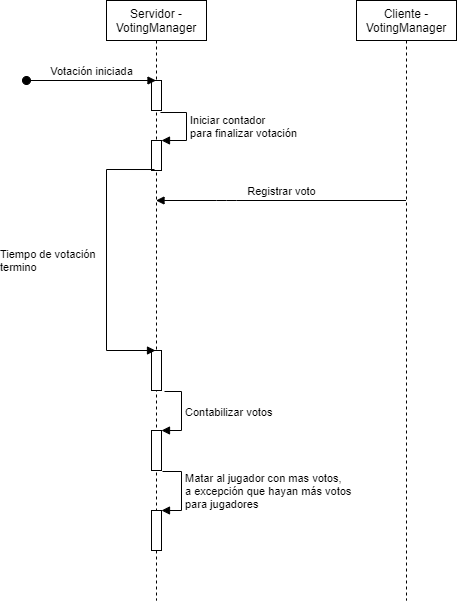
\includegraphics[width=0.5\linewidth]{images/diagrama_secuencia_votos.png}
    \caption{Diagrama de secuencia del sistema de votación}
    \label{fig:diagrama_sec_votacion}
\end{figure}
\begin{figure}[h!]
    \centering
    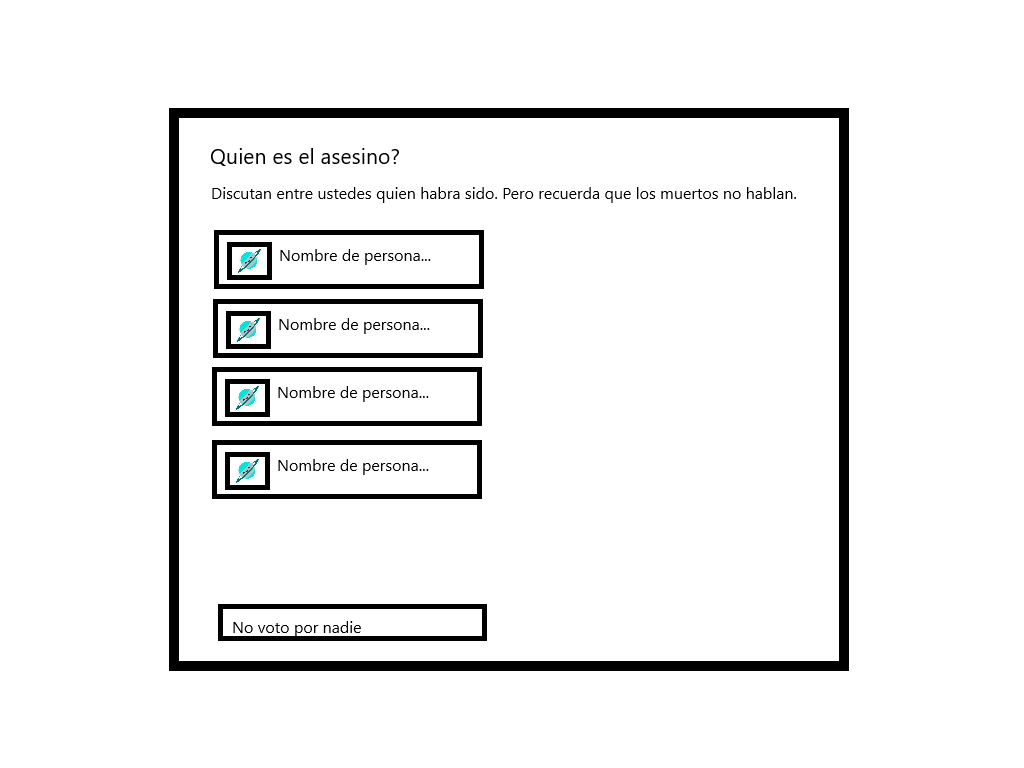
\includegraphics[width=0.5\linewidth]{images/votacion.png}
    \caption{Diseño de interfaz gráfica pantalla de votación de asesinos}
    \label{fig:diagrama_ui_votacion}
\end{figure}

\subsubsection{Modo fantasma}


\subsubsection{Emergencias}
Son tipos especiales de \textit{puzzles}. Tienen la misma complejidad que estos, pero requieren 2 jugadores que los hagan al mismo tiempo para completarlos con éxito. Estos pueden ocurrir varias veces en la partida dependiendo de los asesinos. Estos pueden invocar las emergencias después de un tiempo dado de que haya iniciado la partida, después de un tiempo de juntas y después de un tiempo de que los programadores completaron una primera emergencia correctamente.

Hay tres emergencias disponibles:
\begin{itemize}
    \item Apagar generadores, jugadores tienen que encender un generador de respaldo. En esta emergencia los jugadores necesitan aumentar el valor de un \textit{slider}, haciendo que los jugadores experimenten con un uso potencial de las variables de números enteros (figura~\ref{fig:ui_sab_generador}).
    \begin{figure}[H]
        \centering
        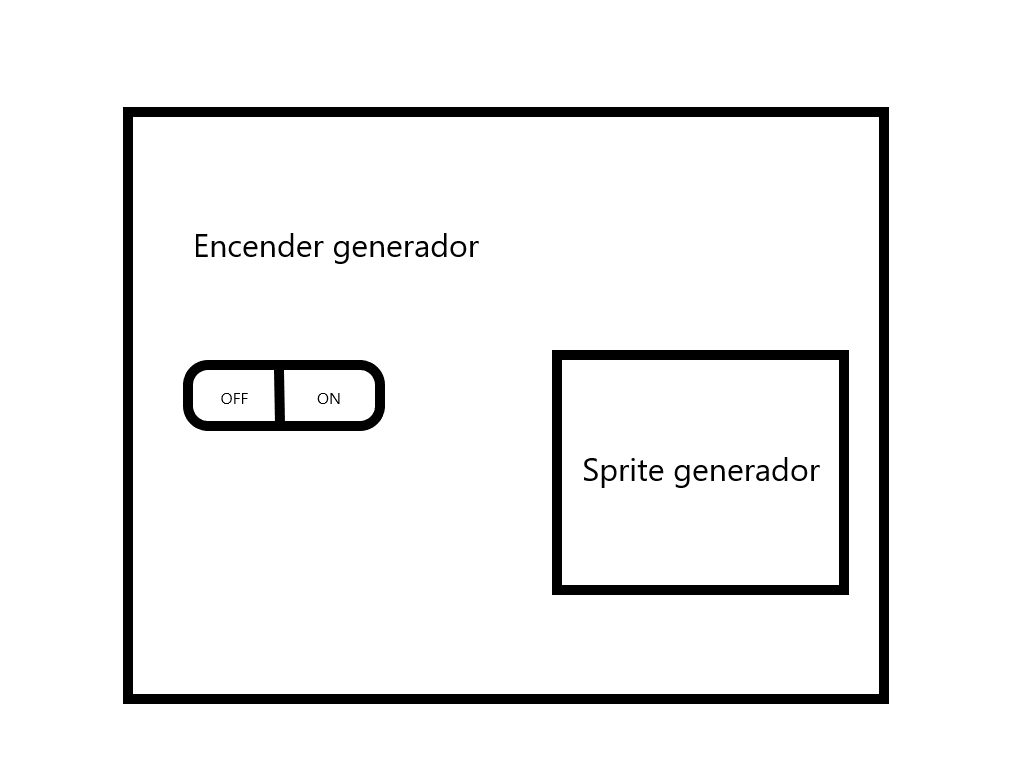
\includegraphics[width=0.5\linewidth]{images/SabotageGenerador.png}
        \caption{Interfaz gráfica de emergencia en los generadores de electricidad}
        \label{fig:ui_sab_generador}
    \end{figure}
    \item Mover presión de \textit{boilers}, jugadores tienen que regular la presión. \textit{Puzzle} consiste en que los jugadores tienen que ver el indicador en pantalla y mantener la presión en verde, modificando el algoritmo en pantalla de forma que mantenga la presión entre el mínimo y el máximo (figura~\ref{fig:ui_sab_presion}).
    \begin{figure}[H]
        \centering
        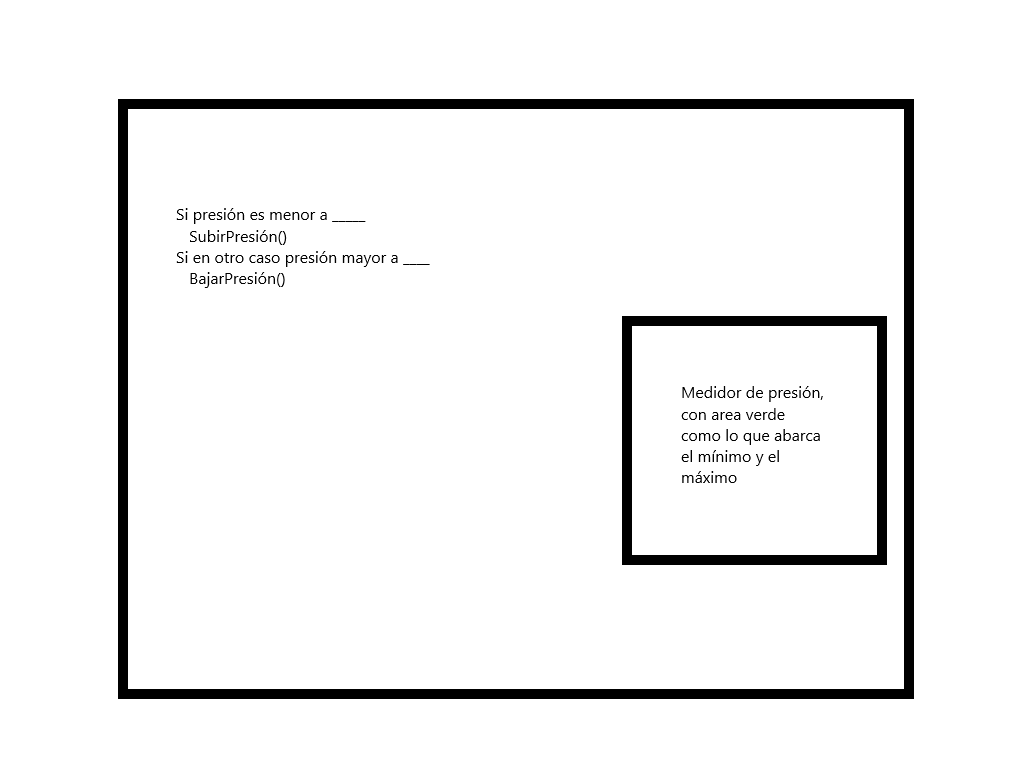
\includegraphics[width=0.5\linewidth]{images/SabotagePresion.png}
        \caption{Interfaz gráfica de emergencia en los boilers}
        \label{fig:ui_sab_presion}
    \end{figure}
    \item Sabotear telégrafo, requiere dos personas contesten preguntas. Al contestar un numero de dado de preguntas correctas resolverán la emergencia. La interfaz gráfica se puede ver en la figura~\ref{fig:ui_teletransporte}.
    \begin{figure}[H]
        \centering
        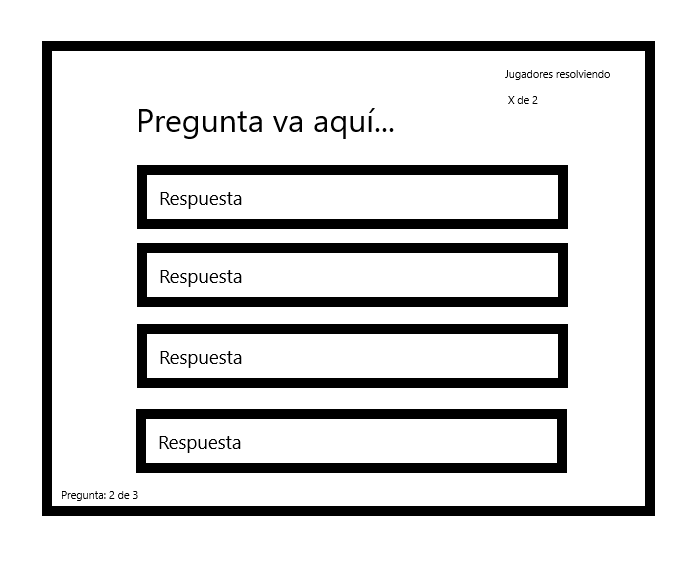
\includegraphics[width=0.5\linewidth]{images/sabotage_preguntas.png}
        \caption{Interfaz gráfica de emergencia de telégrafo}
        \label{fig:ui_teletransporte}
    \end{figure}
\end{itemize}

\subsubsection{Mapa de juego}
\begin{figure}[h]
    \centering
    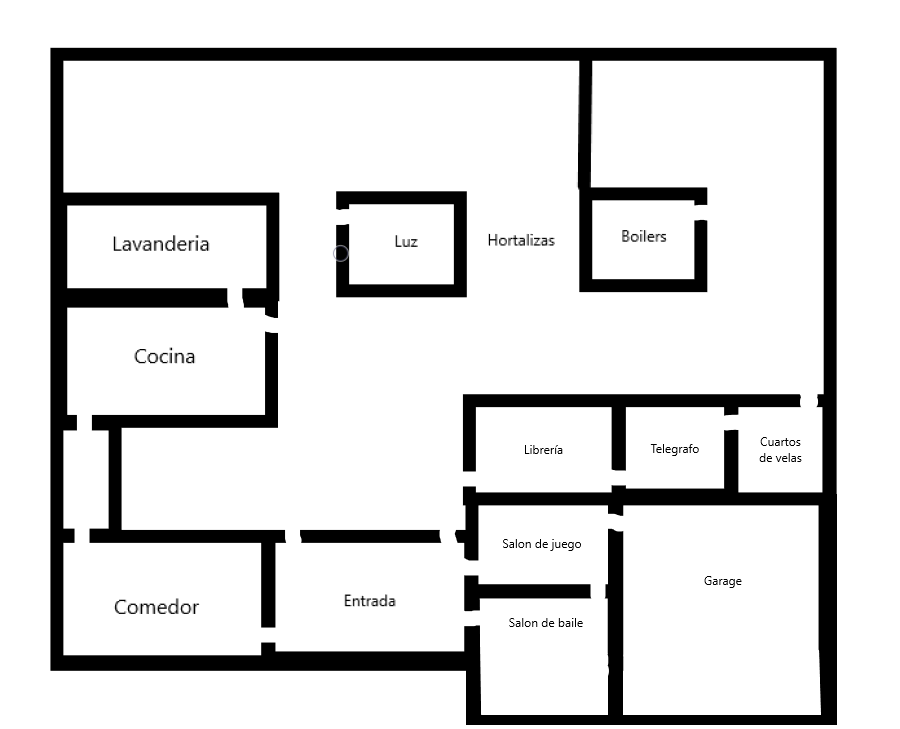
\includegraphics[width=1\linewidth]{images/MapaJuego.png}
    \caption{Organización del mapa del juego}
    \label{fig:mapa_juego}
\end{figure}
El juego se lleva a cabo en una mansión. El mapa consiste en un solo piso. Algunas de las características que se consideró que tuviera el mapa fueron:
\begin{itemize}
    \item Interconectado para permitir a los programadores moverse a completar sus actividades, de preferencia más de una salida entre cuartos. 
    \item Hay algunos cuartos que rompen con la primera regla para los programadores, tienen una sola salida y es muy fácil de que un asesino agarre a un programador haciendo una tarea y fácilmente lo pueda matar. Dado que hay poco flujo de tránsito, la tumba puede quedar no detectada por un rato. La forma de balancear esto es agregando varias tareas en este cuarto de forma que otros jugadores tengan la necesidad de entrar. Algunos jugadores más experimentados dada la reputación de esos cuartos podrán entrar a revisar si no hay ninguna tumba de alguno de sus compañeros programadores.
    \item Áreas grandes principales donde los jugadores circulan a las diferentes salas del juego, normalmente son zonas que un asesino consideraría muy alto riesgo para matar a un programador. Estas son la entrada a la mansión, un patio, el zaguán de atrás de la casa y un patio que conecta los \textit{boilers} con un corral.
\end{itemize}

El diseño del mapa se puede ver en la figura~\ref{fig:mapa_juego}.

\section{Desarrollo}
Usando las libertades dadas por la librería Mirror, se usó el mismo proyecto de Unity para el desarrollo del cliente y el servidor, usando el lenguaje de programación C\#. El servidor se encarga de hospedar las partidas y los clientes que dependen del servidor para manejar el estado. En el fondo la librería se encarga de sincronizar estado además de realizar llamadas y ejecutar funciones RPC a petición del servidor.

El juego se diseñó con un servidor autoritativo, algunos sistemas hacen cálculos en el servidor o las decisiones son rectificadas en este. En sí, el estado del juego será computado mayormente en el servidor, donde el cliente solo estará como un cliente ligero. La comunicación entre estos dos se realizara con el protocolo usando \textit{Websockets} para la transferencia de información, una limitación dada por el soporte de protocolos de comunicación del navegador web.

En esta etapa se realizó la programación de diversos sistemas y comportamientos de distintos elementos del juego.

\subsection{Creación de \textit{sprites} y \textit{assets}}
Según detalles del documento de diseño, se crean los diversos sprites para personajes, animaciones, objetos (mesas, cajas) e interfaces gráficas. Se crearon de todo aquello que no se pudo obtener de spritesheets de uso libre o porque fueron originales para este juego (se hablará de esto más adelante). El diseño de algunos artículos originales se realizó previamente en el documento de diseño del juego. Para los \textit{sprites} se definieron algunas limitantes, como la resolución, donde cada \textit{tile}  tiene medidas de 16x16, el fondo de este es transparente. En los \textit{sprites} necesarios, estuvieron los de personajes jugables (figura~\ref{fig:sprite_johanna}. Estos se diseñaron en \textit{Photoshop}. En el caso de los jugadores miden 1x2 \textit{tiles}. Las mesas (comedor, mesa de billar) son 3x3 \textit{tiles}. 

\begin{figure}[h]
    \centering
    
\includegraphics[width=0.2\linewidth]{images/JohannaOrdonez.png}
    \caption{Sprite de uno de los personajes jugables}
    \label{fig:sprite_johanna}
\end{figure}

Se encontraron \textit{spritesheets} que se pudieran usar con licencia en el proyecto en el sitio web \url{http://itch.io}, esto permitió reducir el trabajo de crear arte para el juego.
Entre estos fueron:
\begin{itemize}
    \item \textbf{Grass++} Variedad de sprites de pastos, flores y misceláneos para los patios y jardines
    \item Platformer 2D Tileset
    \item Dungeon Tileset
    \item Free Tileset Objects - Treasure Chests
\end{itemize}

\subsection{Puzzles}
\begin{itemize}
    \item Variables tipo enteras y variable de punto flotante: Dada la similitud entre ellos se decidió combinar en un solo componente que puede ser reutilizado para ambos. Como se vio anteriormente, este \textit{puzzle} para mostrar un uso posible de las variables de números, se copia la temperatura del termómetro. Acepta entradas de un componente \textit{Slider} o de un \textit{InputField} que de preferencia está configurado para solo números. Se verifica que el resultado sea correcto en el servidor, como se ve en la figura~\ref{fig:diagrama_sec_int_float}.
    \begin{figure}[H]
        \centering
        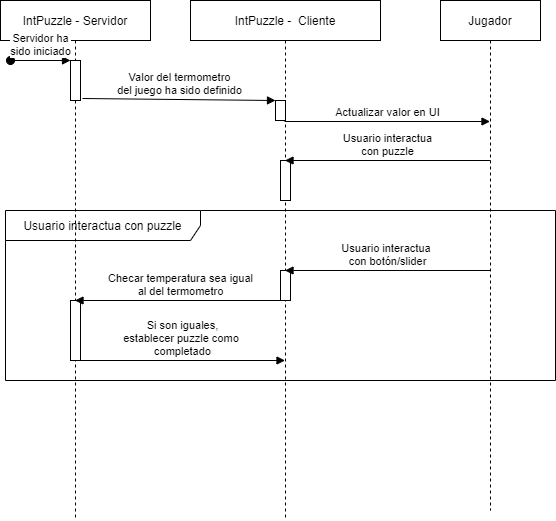
\includegraphics[width=0.8\linewidth]{images/DiagramaSecuenciaPuzzleNumbers.png}
        \caption{Diagrama de secuencia puzzle de int/float}
        \label{fig:diagrama_sec_int_float}
    \end{figure}
    \item Secuencia: Los puzzles de secuencia usan una tabla simulada aprovechando los componentes de \textit{layout} provistos por Unity para el sistema de UI. Se creo un \textit{prefab} para poderlo \textit{spawnear} suficientes cuadritos para el tamaño del campo de juego establecido para el \textit{puzzle}. \texttt{SequenceGrid} es la clase que controla en comportamiento del \textit{puzzle} en el cliente, esta hace las siguiente labores:
    \begin{itemize}
        \item Controles para el jugador
        \item Actualizar sprites del grid cuando hay cambios de posición del jugador
        \item Reiniciar puzzle cuando jugador se cae en un hoyo
    \end{itemize}
    \item Variables tipo string: Un puzzle sencillo para dar un primer al uso de las cadenas string para mostrar en cosas en pantalla, normalmente interpolado con otro texto. La interfaz gráfica del \textit{puzzle} llama una función con el nombre del usuario para que se marque el \textit{puzzle} como completado (figura ~\ref{fig:diagrama_sec_string}) y hacer que un robot cercano le dé la bienvenida mostrando una pequeña burbuja de texto arriba de su cabeza en el juego.
    \begin{figure}[H]
        \centering
        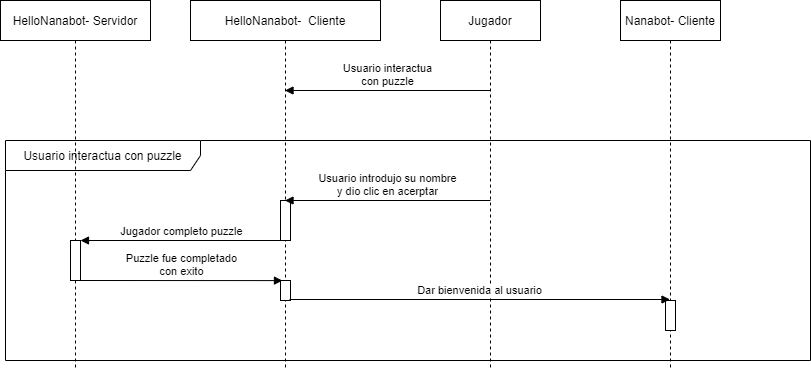
\includegraphics[width=0.8\linewidth]{images/DiagramaSecuenciaPuzzleString.png}
        \caption{Diagrama de secuencia puzzle de cadenas de texto}
        \label{fig:diagrama_sec_string}
    \end{figure}
    \item Variable tipo string - subcadenas: El \textit{puzzle} tiene diferentes subcadenas en cada partida, estos se establecen cuando inicia el servidor. Se calcula el inicio de la subcadena y su longitud. Una vez definido, se llama un \textit{hook} en los clientes para actualizar la UI para que muestren la subcadena a la que los jugadores luego intentaran recrear. Al mover los jugadores \textit{sliders} para cambiar los valores, se calcula cual sería la subcadena formada y se mantiene el estado en el cliente, aunque se manda una copia al servidor para validar que si es el resultado esperado, en el caso que lo sea, se considera el \textit{puzzle} como terminado (figura~\ref{fig:diagrama_sec_subcadena}).
    \begin{figure}[H]
        \centering
        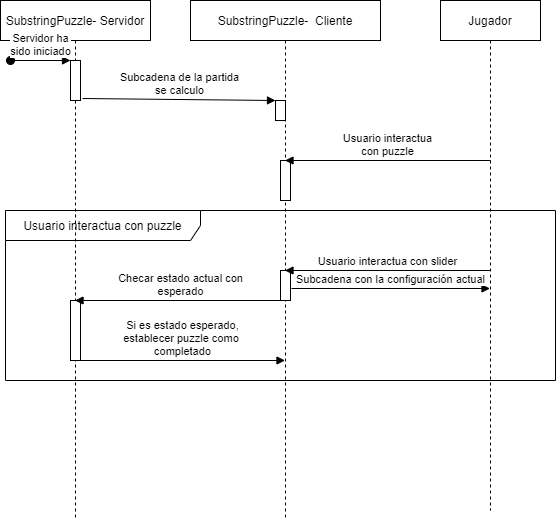
\includegraphics[width=0.8\linewidth]{images/DiagramaSecuenciaPuzzleSubstring.png}
        \caption{Diagrama de secuencia puzzle de subcadena}
        \label{fig:diagrama_sec_subcadena}
    \end{figure}
    \item  Variables tipo booleano: Como solo depende de un botón para cambiar el estado, \textit{CompleteBoolPuzzle} tiene una función pública en el cliente que llama la UI cuando se enciende que llama al servidor para indicar que se completó el \textit{puzzle} (figura~\ref{fig:diagrama_sec_booleano}) y marcarlo como tal para los demás jugadores.
    \begin{figure}[H]
        \centering
        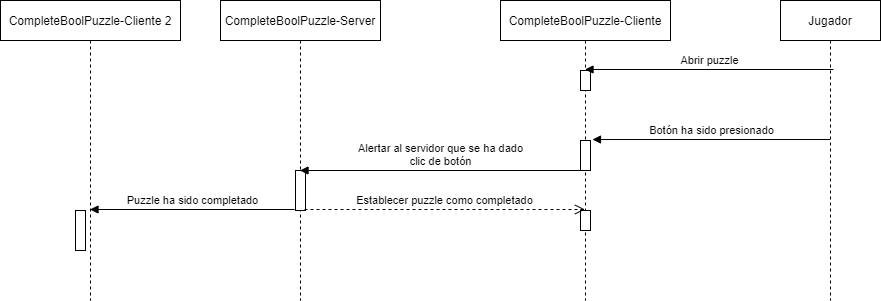
\includegraphics[width=0.8\linewidth]{images/DiagramaSecuenciaPuzzleBool.png}
        \caption{Diagrama de secuencia puzzle de subcadena}
        \label{fig:diagrama_sec_booleano}
    \end{figure}
    \item Do While: El \textit{puzzle} es simple en lógica, no necesita crear valores aleatorios o seleccionar que configuración de una lista elegir. Existe un componente \texttt{InputField} para que el jugador pueda  configurar una variable booleana, el valor de este  se revisa en el servidor para asegurarse que fue completado (figura~\ref{fig:diagrama_sec_do_while}).
    \begin{figure}[H]
        \centering
        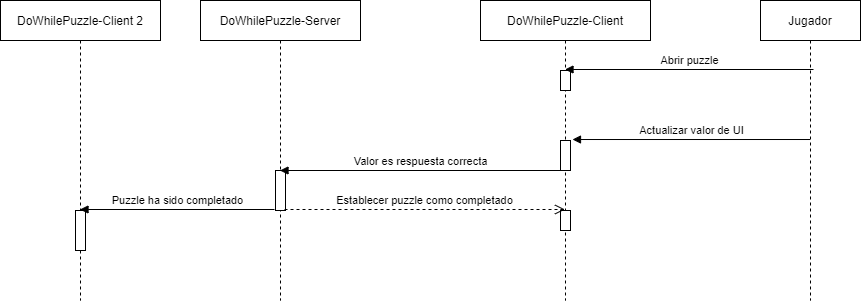
\includegraphics[width=0.8\linewidth]{images/DiagramaSecuenciaPuzzleDoWhile.png}
        \caption{Diagrama de secuencia puzzle do while}
        \label{fig:diagrama_sec_do_while}
    \end{figure}
    \item Ciclo tipo for: Este \textit{puzzle} cada vez que se ejecuta requiere un numero aleatorio que define el número de iteraciones que necesita el algoritmo que completa el usuario, este valor se pasa del servidor a cada cliente al iniciar el servidor, cuando el jugador mete un valor, se verifica en el servidor de que la entrada sea el valor correcto para completarlo (figura~\ref{fig:diagrama_sec_for}).
    \begin{figure}[H]
        \centering
        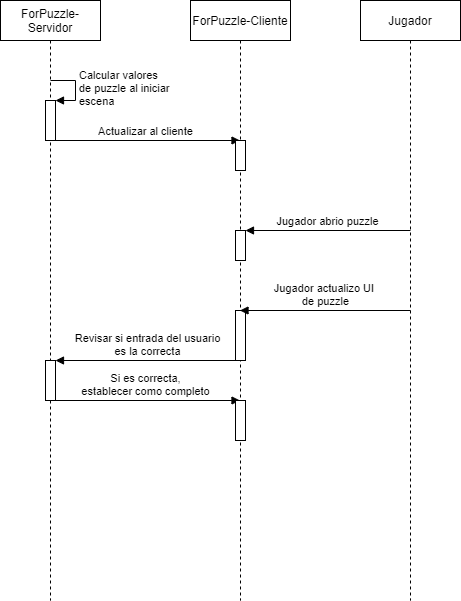
\includegraphics[width=0.4\linewidth]{images/DiagramaSecuenciaPuzzleFor.png}
        \caption{Diagrama de secuencia puzzle for}
        \label{fig:diagrama_sec_for}
    \end{figure}
    \item Ciclo tipo while: Su única tarea es revisar que el valor de llenado de la cubeta introducido por el usuario sea el valor correcto, que está definido en 6 (figura~\ref{fig:diagrama_sec_while}).
    \begin{figure}[H]
        \centering
        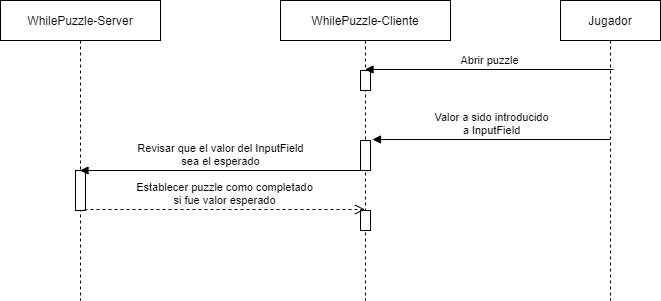
\includegraphics[width=0.8\linewidth]{images/DiagramaSecuenciaPuzzleWhile.png}
        \caption{Diagrama de secuencia puzzle while}
        \label{fig:diagrama_sec_while}
    \end{figure}
    \item If: Para la creación de los botones con imágenes de las flores para la selección de la flor que hay que selecciona se creó un componente que sirva como abstracción, que se conecta con los componentes de \texttt{Button} y \texttt{Image} y ofrece propiedades para facilitar cambiar cosas del botón sin depender de los componentes usados en la implementación. 
    Antes de que cualquier jugador pueda interactuar con el \textit{puzzle}, del lado del servidor se decide la flor que debe agarrar en jugador de manera aleatoria. Después de decidirse esta flor, se manda su \textit{id} codificado como una enumeración al cliente y el cliente recibe en un \textit{hook} este y actualiza la imagen del código del \textit{if} para mostrar la flor que el jugador tiene que seleccionar. 
    Una vez que el jugador interactúa con el \textit{puzzle}, se manda el clic del botón con el id a la flor que corresponden, si el usuario selecciona el correcto se cuenta como que se completó el \textit{puzzle}, y un subsistema se encarga de aumentar el contador (figura~\ref{fig:diagrama_sec_if}).
    \begin{figure}[H]
        \centering
        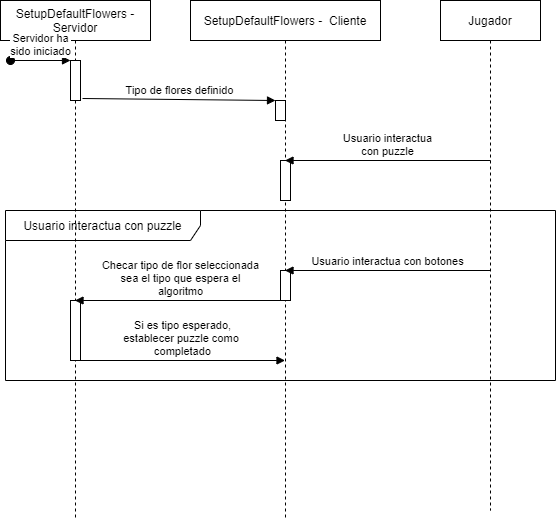
\includegraphics[width=0.8\linewidth]{images/DiagramaSecuenciaPuzzleIf.png}
        \caption{Diagrama de secuencia puzzle if}
        \label{fig:diagrama_sec_if}
    \end{figure}
    \item If/else: El \textit{puzzle if/else} necesita un valor aleatorio que se calcula cuando inicia el servidor, este valor es usado para decidir si se va a decorar un pastel o un \textit{cupcake}, como se había visto anteriormente le mostramos al jugador un pseudocódigo de la forma que debería de decorar el postre. Y el jugador tiene un \textit{sprite} del postre a decorar y selecciona con dos botones inferiores la decoración a usar. Al calcularse este valor anterior en el servidor, Mirror llama un \textit{hook} en el cliente sobre el cambio del valor de la variable, usamos este \textit{hook} para cambiar el \textit{sprite} del postre a decorar (figura~\ref{fig:diagrama_sec_if_else}).
    Para marcar el \textit{puzzle} como completado, hay unas funciones especiales que mandan la selección de decoración al servidor y si es la decoración correcta marcan el \textit{puzzle} como completado.
    \begin{figure}[H]
        \centering
        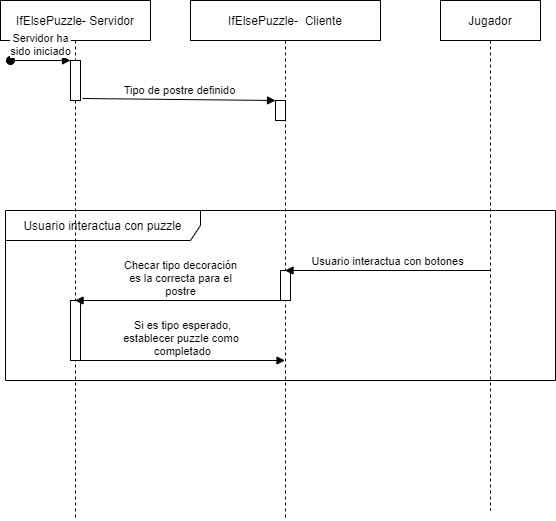
\includegraphics[width=0.8\linewidth]{images/DiagramaSecuenciaPuzzleIfElse.png}
        \caption{Diagrama de secuencia puzzle if else}
        \label{fig:diagrama_sec_if_else}
    \end{figure}
\end{itemize}

\subsection{Sistema de versiones}
Para la elaboración del proyecto se usó el sistema de versiones Git. El repositorio es público y puede ser accedido en \url{https://github.com/SaulNunez/Project-Hamilton}.

\subsection{Integración Continua}
Se usó Github Actions permite ejecutar un \textit{script} después de crear nuevos \textit{commits} a la rama \textit{Master}.
Ejecuta las siguientes acciones cada vez que se activa el trabajo:
\begin{itemize}
    \item Compila ejecutables para Windows x64-86 y WebGL
    \item Crea documentación de las funciones y variables del proyecto y sube usando \textit{Github Pages} la nueva versión a la página \url{http://saulnunez.com/Project-Hamilton/}
\end{itemize}

Para la compilación de ejecutables se usó el increíble trabajo de GameCI que tiene imágenes preconfiguradas de Unity que facilitan la creación de los \textit{pipelines} necesarios para la compilación. Se uso su tutorial disponible en \url{https://game.ci/docs/github/v1/builder} y sus ejemplos para la creación del \textit{script}.

En la creación del pipeline de la generación de documentación se usó el trabajo de Normand Erwan disponible en \url{https://github.com/NormandErwan/DocFxForUnity} que provee la configuración de DocFX para que funcione con la organización por carpetas de Unity y por la forma en la que este de manera predefinida crea clases para componentes en el \textit{namespace} \textbf{global}.

\section{Implementación}
\subsection{Sprites}
Como lo vimos anteriormente, hay dos tipos de \textit{sprites}. Aquellos que se obtuvieron de itch.io se agregaron simplemente a Unity importándolos a las carpetas del proyecto y configurado para que los interpretara como \textit{"sprites"}, estos al ser \textit{spritesheets} (y por lo tanto contener en un solo archivo un numero de \textit{sprites} individuales) se cortan en el editor de \textit{sprites} dependiendo del tamaño en el que fueron diseñados (normalmente 16x16 o 32x32 píxeles); normalmente aquí acabaría el proceso pero en algunos sprites requirieron ajustes manuales por su forma de \textit{"sprite packing"} (como se organizan los sprites entre el archivo de imagen). En el segundo tipo, fueron los creados específicamente para el juego, estos fueron diseñados en Photoshop, se usó el \textit{plugin} de PSDs para permitir importar archivos de Photoshop directamente a Unity para utilizarlos, dependiendo de la situación del \textit{sprite} en particular se dejaba en simple o en múltiples, estos últimos cortados en  16x16 para ítem grandes que usan el principio 9-slice.

\subsection{Emergencias}
Para las emergencias se decidió crear un subsistema para controlar su estado. Este controla la interfaz que tienen los impostores para encender las emergencias. Así como los \textit{timeouts} necesarios para que las emergencias tarden un tiempo determinado antes de poder ser activados cuando inicia el juego y cuando se reinicia el contador por una votación para sacar a alguien o por el \textit{cooldown} a una emergencia previa.
Como los emergencias incluyen acciones comunes como activarlos o detenerlos, se creó una clase base que usan todos estos para incluir estos métodos (figura~\ref{fig:diagrama_clases_emergencias}).
\begin{figure}[h]
    \centering
    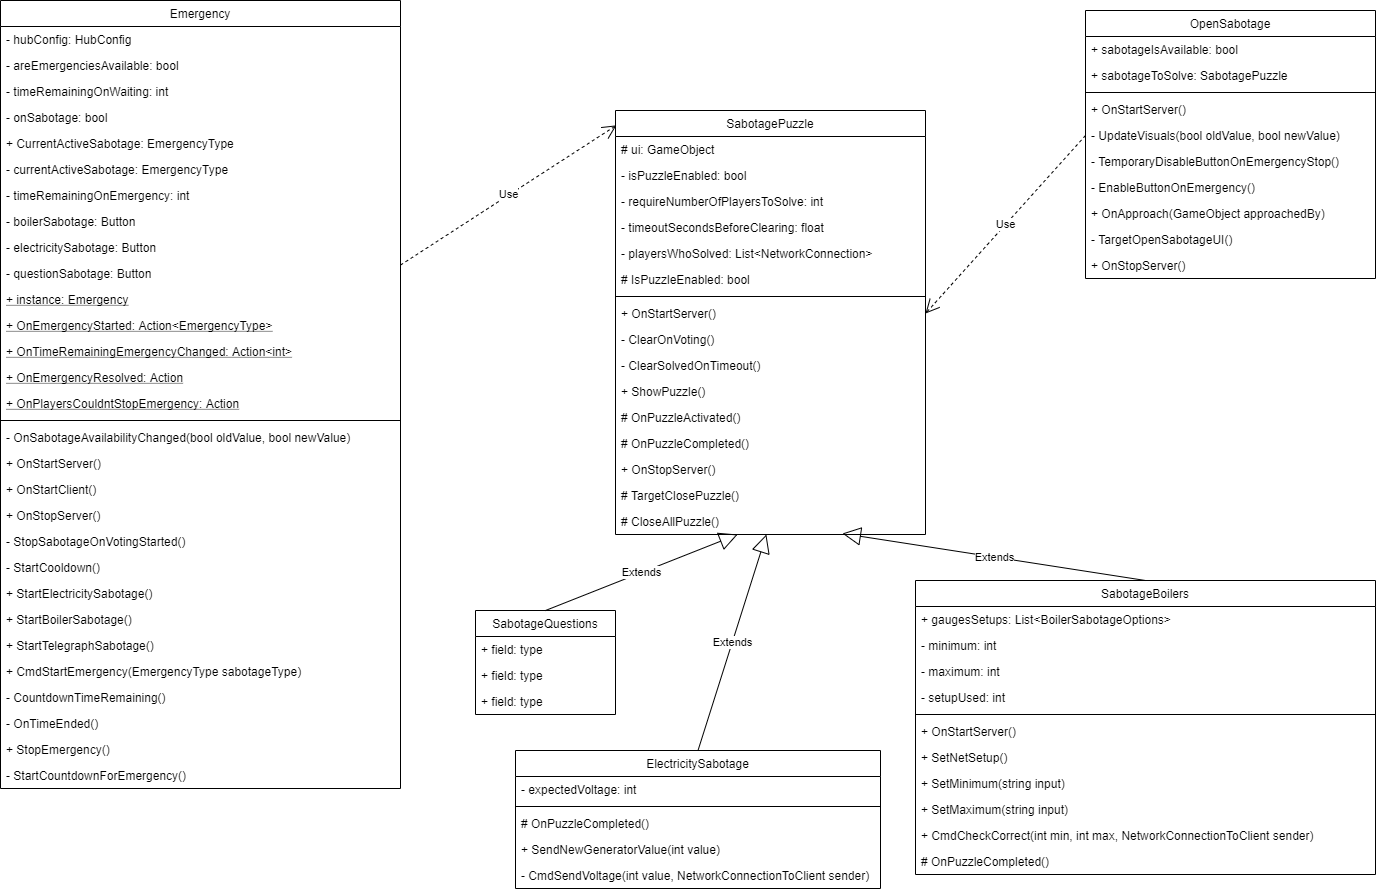
\includegraphics[width=1\linewidth]{images/DiagramaClasesEmergencias.png}
    \caption{Diagrama de clases del sistema de emergencias}
    \label{fig:diagrama_clases_emergencias}
\end{figure}
\begin{itemize}
    \item Emergencia de telégrafo, la selección de pregunta y su revisión ocurren en el servidor, el cliente recibe información sobre la pregunta actual (para mostrarla en pantalla) y todo mundo(como todos los que están respondiendo el emergencia, mínimo los dos jugadores) tiene que contestar la pregunta actual para poder pasar a la siguiente, como se ve en la figura~\ref{fig:diagrama_secuencia_emergencia_pregunta}.
        \begin{figure}[h]
            \centering
            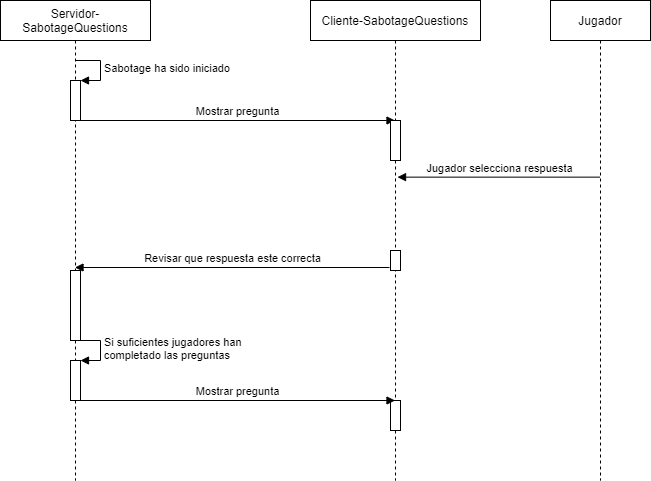
\includegraphics[width=1\linewidth]{images/diagrama_secuencia_sabotage_preguntas.png}
            \caption{Diagrama de secuencia de emergencia de telégrafo}
            \label{fig:diagrama_secuencia_emergencia_pregunta}
        \end{figure}
    \item Apagar generadores, la única función que realiza el cliente es mandar la nueva posición del \textit{slider} al servidor, como se puede ver en la figura~\ref{fig:diagrama_secuencia_generadores}.
        \begin{figure}[h]
            \centering
            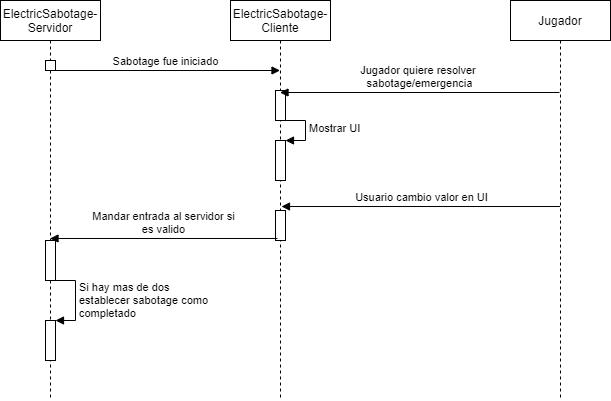
\includegraphics[width=1\linewidth]{images/DiagramaSecuenciaSabotageGeneradores.png}
            \caption{Diagrama de secuencia de emergencia en los generadores}
            \label{fig:diagrama_secuencia_generadores}
        \end{figure}
    \item Ajustar presión del boiler, hay distintos medidores de los cuales elige uno para mostrar por emergencia, al definirse uno, se actualiza la UI en el cliente, cada vez que el jugador juegue con los valores del algoritmo que el usuario necesita completar para regular la presión se revisara en el cliente que son el valor ideal.
\end{itemize}

\subsection{Despliegue}
Se crearon varias imágenes \textit{Docker} para hospedar los programas del cliente y servidor. Estos contenedores son manejados por \textit{Docker Compose} que controla su estado y crea una red local simulada entre estos. El diagrama de la conexión entre los contenedores y el mundo real se puede ver en la figura~\ref{fig:diagrama_despliege}, el \textit{stack} de red del servidor manda los paquetes de red a Docker que a la vez la delega a los contenedores.
En el caso específico del cliente que corre cada usuario se usó Apache para el \textit{host} de los archivos estáticos.
Para la configuración del servidor en \textit{Ubuntu} se llevó a cabo según las guías de Mirror networking, disponibles en: \url{https://mirror-networking.gitbook.io/docs/guides/server-hosting/google-cloud}, sobre un contenedor que corre Ubuntu.
El protocolo usado para la comunicación se usó \textit{websockets}, para poder usar la misma dirección y el mismo puerto 80 que el sitio como para realizar la conexión al servidor (\url{http://pruebas.saulnunez.com} para el cliente y \url{ws://pruebas.saulnunez.com} para el servidor), se usó Apache como servidor Proxy, el cual hace redirección al servidor que contiene el sitio del cliente si el protocolo es http, pero si tiene el /texit{header} para hacer \texit{upgrade}se dirige al servidor de juego.
Para hospedar todo se usó \textit{Ubuntu} en \textit{Google Cloud Compute Engine}, en el cual para instalar Docker que uso la guía de instalación oficial: \url{https://docs.docker.com/engine/install/ubuntu/}. Docker Compose se necesitó instalar por separado, lo que se realizó con su guía oficial de instalación, obtenida aquí: \url{https://docs.docker.com/compose/install/}.

\begin{figure}[h]
    \centering
    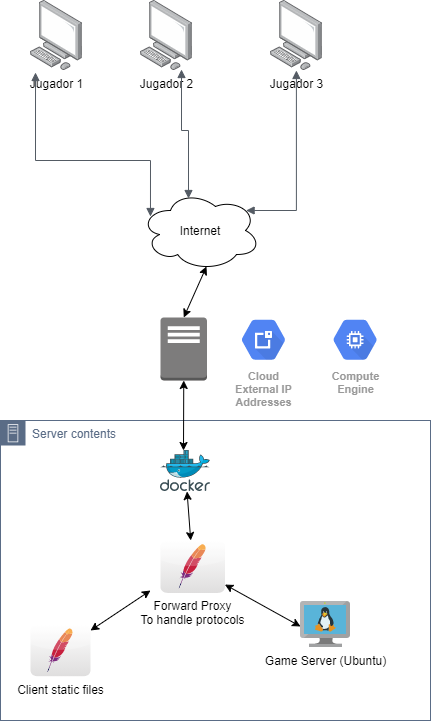
\includegraphics[width=0.5\linewidth]{images/diagrama_deployment.png}
    \caption{Diagrama del despliegue}
    \label{fig:diagrama_despliege}
\end{figure}

\section{Pruebas}
Durante el desarrollo se usaron pruebas de humo en el producto, se usó el \textit{asset} \href{https://github.com/hwaet/UnityProjectCloner}{UnityProjectCloner} para crear una copia del proyecto para poder simular en la misma computadora un cliente y lo que la librería Mirror llama un \textit{host}, un cliente con el servidor integrado, a base de esto poder probar que el código generado tenía el funcionamiento esperado y que no tuviera errores o problemas de configuración. Fueron pruebas de 5-15 minutos sobre el sistema que se estaba trabajando en ese momento.

Se hicieron tres \textit{soak tests} distintos. Uno se dejó durante 3 horas la pantalla de inicio, en el segundo se dejó el \textit{lobby} y en la tercera una sesión del juego.

Se hicieron pruebas de funcionalidad en una ocasión, con 3 jugadores para revisar la usabilidad de la interfaz gráfica, ver la estabilidad y ver problemas en las mecánicas del juego.

En el despliegue, se realizaron pruebas de integración de manera manual a fin de detectar que se conectara correctamente el cliente y el servidor. Debido a el uso de los contenedores de \textit{Docker} no se tuvo que hacer pruebas para compensar las diferencias de configuración entre el entorno de pruebas y el sistema final, dado que es exactamente el mismo. Adicionalmente se realizó una sesión donde se simulo una partida con tres jugadores para hacer pruebas del multijugador con el servidor para ver si ocurrían problemas debido a la latencia entre el cliente y el servidor debido a la distancia de la conexión con el servidor.
